% =====================================================================
% genomic-semiotic-graph-verditcs.tex
%
% Genomic Semiotic Graph Verdicts.
% A self-contained manuscript. It derives the theory it needs and cites
% only external literature. Every number in Part IV is read from
% validation/results/*.json, written by the scripts in validation/.
% =====================================================================

\documentclass[11pt,twocolumn,a4paper]{article}

\usepackage[T1]{fontenc}
\usepackage[utf8]{inputenc}
\usepackage{lmodern}
\usepackage[margin=2.3cm]{geometry}
\usepackage{amsmath,amssymb,amsthm,mathtools}
\usepackage{booktabs}
\usepackage{array}
\usepackage{graphicx}
\usepackage{caption}
\captionsetup{font=small,labelfont=bf}
\usepackage{enumitem}
\usepackage{xcolor}
\usepackage{listings}
\usepackage[expansion=false]{microtype}
\usepackage[hidelinks]{hyperref}
\usepackage[capitalise,nameinlink]{cleveref}
\usepackage[numbers,sort&compress]{natbib}
\bibliographystyle{unsrtnat}

\setlist{leftmargin=1.5em,itemsep=1pt,topsep=3pt}
\newcolumntype{L}[1]{>{\raggedright\arraybackslash}p{#1}}

% ---------------------------------------------------------------------
\theoremstyle{plain}
\newtheorem{theorem}{Theorem}[section]
\newtheorem{proposition}[theorem]{Proposition}
\newtheorem{lemma}[theorem]{Lemma}
\newtheorem{corollary}[theorem]{Corollary}
\theoremstyle{definition}
\newtheorem{definition}[theorem]{Definition}
\newtheorem{construction}[theorem]{Construction}
\newtheorem{assumption}[theorem]{Assumption}
\theoremstyle{remark}
\newtheorem{remark}[theorem]{Remark}
\crefname{assumption}{Assumption}{Assumptions}
\crefname{construction}{Construction}{Constructions}

% ---------------------------------------------------------------------
\newcommand{\U}{\mathcal{U}}
\newcommand{\Kc}{\mathcal{K}}
\newcommand{\Sig}{\Sigma}
\newcommand{\Opn}{\Omega}
\newcommand{\Ind}{\mathrm{I}}
\newcommand{\cp}{\mathord{+}}
\newcommand{\cm}{\mathord{-}}
\newcommand{\cz}{\mathord{\bot}}
\newcommand{\G}{G}
\newcommand{\Iset}{\mathsf{I}}
\newcommand{\Zset}{\mathsf{Z}}
\newcommand{\Lset}{\mathsf{L}}
\newcommand{\Tset}{\mathsf{T}}
\newcommand{\Vars}{\mathsf{X}}
\newcommand{\Pc}{P_{\mathrm{c}}}
\newcommand{\Pp}{P_{\mathrm{p}}}
\newcommand{\Desc}{V}
\newcommand{\Qfrag}{\mathcal{Q}_{\mathrm{b}}}
\newcommand{\ans}{\mathrm{ans}}
\newcommand{\Aut}{\mathrm{Aut}}
\newcommand{\orb}{\mathrm{Orb}}
\newcommand{\dom}{\mathrm{dom}}
\newcommand{\Act}{\mathrm{Act}}
\newcommand{\gr}{\gamma}
\newcommand{\vsym}{\textsf{symbol}}
\newcommand{\vcol}{\textsf{collapsed}}
\newcommand{\vind}{\textsf{index}}
\newcommand{\vico}{\textsf{icon}}
\newcommand{\vcom}{\textsf{composite}}
\newcommand{\genby}{\texttt{prov:wasGeneratedBy}}
\newcommand{\used}{\texttt{prov:used}}
\newcommand{\assoc}{\texttt{prov:wasAssociatedWith}}
\newcommand{\rdftype}{\texttt{rdf:type}}
\newcommand{\la}{\mathtt{a}}
\newcommand{\lp}{\mathtt{+}}
\newcommand{\lm}{\mathtt{-}}
\newcommand{\Vis}{\mathcal{V}}
\newcommand{\Rnn}{\mathbb{R}_{\ge0}}

\lstdefinestyle{ttl}{basicstyle=\ttfamily\scriptsize,columns=fullflexible,
  breaklines=true,frame=single,rulecolor=\color{black!25},xleftmargin=2pt,
  framesep=3pt,showstringspaces=false}

\hypersetup{pdftitle={Genomic Semiotic Graph Verdicts}}

% =====================================================================
\title{\textbf{Genomic Semiotic Graph Verdicts}\\[0.3em]
\large Content, Ground, and the Witnessed Outside of a Genomic Record}

\author{%
Kundai Farai Sachikonye\\[0.3em]
\normalsize Experimental Bioinformatics, TUM School of Life Sciences\\
\normalsize AIMe Registry for Artificial Intelligence\\
\normalsize Maximus-von-Imhof-Forum 3, 85354 Freising, Germany\\
\normalsize \texttt{kundai.sachikonye@bitspark.com}}

\date{\today}

\begin{document}
\maketitle

% =====================================================================
\begin{abstract}
\noindent
A genomic record---a genotype call, a gene--term annotation, a clinical
classification of a variant---can say the same thing as another record while
standing in an entirely different relation to what it describes. A genotype
read from sequencing reads and a genotype imputed from a reference panel can
carry the same value; an annotation from a direct assay and one inferred
electronically can attach the same gene to the same term; a classification
from clinical testing and one taken from the literature can agree. A query
that returns rows returns them alike. We call what a record says its
\emph{content} and what the graph records about how it came to be its
\emph{ground}, following Peirce's distinction between an index, connected to
its object by contact, and an icon, which shares its object's form. A second
distinction runs alongside it: a record asserts the inside of a distinction
and leaves the outside open, so that an absent genotype call may mean a
reference genotype or an unread position.

We develop the theory from first principles and test every finite claim. On
the outside of records we prove a three-valued calculus in which a pair of
samples is certified different, open, or indiscernible; that certification by
single-valued calls is permanent under growth; that open pairs are exactly
undetermined calls; and that the four common emissions of a cohort---variant-%
only, joint-called, reference-blocked and imputed---form a chain along which
certification only grows, while imputation introduces certificates whose ground
is a derivation and which can be false. On the ground of records we prove,
for an identifier-blind fragment of SPARQL, genericity, an exact orbit
characterisation, predicate locality and content blindness; define
\emph{semiotic verdicts} (\vsym, \vcol, \vind, \vico, \vcom) as a least fixed
point; and prove them definable by three property-path queries, monotone under
growth, sound under truthful emission and independent of content. For identity
across the type/token divide we prove that the magnitude-spectrum receiver used
for alignment-free sequence search is invariant under rotation and reversal,
that the matched-filter receiver is injective, and that corroboration at a
declared floor never identifies beyond a receiver's fibre.

Seven experiments test the claims, four of them on public data. Over
$407{,}232$ exhaustively enumerated sample pairs the calculus holds without
exception; over $2{,}640$ renamed graphs eleven query classes show $0$
genericity violations against $211$, $170$ and $240$ of $240$ for three
controls; and $160/160$ pairs agree between graph automorphism and the
description query. Three genomics LinkML schemas (MIxS, GHGA, NMDC) emit every
class and slot under its own IRI ($\Lambda=0$), against $57$ and $14$ class
distinctions lost by two chemistry profiles; MIxS declares no activity class at
all and writes method and software into $54$ content slots. On $585{,}235$
gene--term memberships of the human, yeast and \emph{Arabidopsis} Gene
Ontology annotations and $4{,}404{,}748$ ClinVar variants, verdicts computed by
SPARQL agree with the fixed point in every sampled record; across $22$
chronological ingestion steps of $6{,}735{,}018$ ClinVar submissions no verdict
falls while $18{,}493$ variants leave the pathogenic class. The median human
GO term with at least twenty genes has $59\%$ of its members without
experimental ground, $74\%$ in \emph{Arabidopsis}; a gene-set file returns the
same members with $1.74$ bits of ground per record erased, and a VCF-style
emission of ClinVar keeps $0.08$ of $0.20$ bits. Exhaustively over all
sequences of length $4$--$10$, $29$--$56\%$ lie in magnitude-spectrum fibres
strictly larger than their rotation--reversal orbit. Content and ground are
independent, and only the ground that is written survives.
\end{abstract}

\tableofcontents

% =====================================================================
\section{Introduction}
\label{sec:intro}
% =====================================================================

\subsection{Three pairs of records}

Consider three pairs of records, each of which is common in genomic
practice.

\begin{enumerate}[label=(\roman*)]
\item \textbf{A genotype.} A sample's genotype at a single-nucleotide
  variant is called from aligned reads \citep{mckenna2010,danecek2021}. In a
  second sample the same position was not covered, and its genotype is imputed
  from a haplotype reference panel
  \citep{li2003,marchini2010,das2016,browning2016}. Both records state
  \texttt{GT=0/1} at the same variant. Merged into one cohort file, they are
  two rows of the same form.
\item \textbf{A gene--term annotation.} A gene is annotated to a Gene
  Ontology term \citep{ashburner2000,go2023} with the evidence code IDA,
  inferred from direct assay; another is annotated to the same term with IEA,
  inferred from electronic annotation. A gene-set file used for enrichment
  analysis \citep{subramanian2005,liberzon2011} lists both genes under the
  term, without evidence.
\item \textbf{A clinical classification.} A variant is classified
  pathogenic in ClinVar \citep{landrum2018} by a laboratory that tested a
  patient's sample; another is classified pathogenic by a submitter whose
  collection method is \emph{literature only}. A query for pathogenic variants
  in the gene returns both.
\end{enumerate}

Each pair agrees in what it says and differs in how it came to say it. One
member of each pair was produced by bringing an instrument into contact with a
material sample; the other was computed from other records. Whether the two
members are ``the same'' is decided in practice, again and again, by whatever
the query language and the file format happen to preserve.

\subsection{Content and ground; inside and outside}

We separate two readings of a record. Its \emph{content} is what it asserts
about its object: the genotype, the term, the classification. Its
\emph{ground} is what the graph records about how it came to be: the activity
that generated it, what that activity used, and who or what carried it out.
The distinction is Peirce's \citep{peirce_cp,peirce1906}. An \emph{index}
signifies by a real, causal connection to its object; an \emph{icon} by sharing
its form; a \emph{symbol} by convention. A called genotype is an index of the
sample whose reads produced it. An imputed genotype is an icon of the panel
haplotypes it was copied from. An identifier is a symbol.

A second distinction is independent of the first. A record asserts the
\emph{inside} of a distinction---this sample carries the alternative allele---and
leaves the \emph{outside} open. Under the open-world reading of the Semantic
Web \citep{rdf11,hogan2021}, and in the variant call format
\citep{danecek2011}, the absence of a non-reference call does not assert a
reference genotype. A site-only or variant-only file cannot distinguish a
sample that was sequenced and found homozygous for the reference from a sample
that was never read there. Reference blocks in a genomic VCF \citep{poplin2018}
exist to write that difference, and imputation exists to fill it.

\subsection{What this paper shows}

We develop the theory needed to state these differences exactly, and test it.

\begin{enumerate}
\item \textbf{Calls as three-valued distinctions} (\Cref{sec:calls}). A pair of
  samples is certified different, open, or indiscernible; certification by a
  single-valued call is permanent under growth; open pairs are exactly
  undetermined calls (\Cref{thm:trichotomy,thm:growth,prop:open}). The
  variant-only, joint-called, reference-blocked and imputed emissions of a
  cohort form a chain along which certification only grows
  (\Cref{prop:chain}); truthful emissions certify only true differences, and
  imputed certificates can be false (\Cref{prop:truthful}).
\item \textbf{Genericity and orbits} (\Cref{sec:generic}). For an
  identifier-blind fragment of SPARQL~1.1, every query commutes with every
  renaming of samples, calls and activities; two individuals are separated by
  some query exactly when no automorphism maps one to the other; and a query
  sees only the predicates it names (\Cref{thm:generic,thm:orbit,prop:locality}).
\item \textbf{Receivers} (\Cref{sec:receivers}). A schema, a file format and an
  embedding are receivers: functions of the record through which every later
  reader sees it. A coarser receiver sees larger cells
  (\Cref{prop:factor}); distinctions drawn only by class are lost when classes
  share an IRI (\Cref{thm:collapse}).
\item \textbf{Semiotic verdicts} (\Cref{sec:verdicts}). The ground of a
  record is a least fixed point with five values. Verdicts are definable by
  three property-path queries, monotone, sound under truthful emission, and
  independent of content (\Cref{thm:definable,thm:monotone,cor:sound,prop:independent}).
\item \textbf{Twins} (\Cref{sec:twins}). A sequenced and an imputed call with
  equal content are separable exactly when the emitted provenance breaks
  their symmetry, with an exact law for incomplete emission
  (\Cref{prop:twinprob}).
\item \textbf{Identity at a declared floor} (\Cref{sec:floor}). The
  magnitude-spectrum receiver of alignment-free search is invariant under
  rotation and reversal; the matched-filter receiver is injective; a strand
  receiver identifies the two strands of a duplex
  (\Cref{thm:dihedral,thm:phase,prop:strand}).
\item \textbf{Answering} (\Cref{sec:answering}). The grounding profile of an
  answer is not a function of the answer (\Cref{thm:profilefree}).
\item \textbf{Validation} (\Cref{sec:validation}). Seven experiments, four on
  public data: three GO annotation sets, the full ClinVar submission summary,
  and five LinkML schemas.
\end{enumerate}

\subsection{What is not claimed}

The theorems concern what a graph, a query fragment and a receiver can
distinguish, not what is true of a genome. We do not claim that called
genotypes are more accurate than imputed ones, that experimental GO evidence is
more reliable than electronic inference, or that a ClinVar classification from
clinical testing is more correct than one from the literature; each can be
wrong. A verdict certifies what the emitted graph says about a record's
generation, not the world: under fabrication it is wrong by construction
(\Cref{prop:fabricate}). The witness declarations that assign evidence codes
and collection methods to contact and derivation are inputs of the method
(\Cref{tab:declarations}), not facts derived from the data, and we report how a
second declaration changes the ClinVar results.

% =====================================================================
\section{Semiotic preliminaries}
\label{sec:semiotics}
% =====================================================================

For Peirce a sign is a relation among a representamen (the sign vehicle), an
object, and an interpretant \citep{peirce_cp}. The object is double: the
\emph{immediate} object is the object as the sign represents it, the
\emph{dynamical} object is the object that determines the sign. In a genomic
graph the record is the representamen, its content is the immediate object,
and the sample, the reads or the molecule is the dynamical object, which no
graph contains. What a graph can contain is a record of how the dynamical
object determined the sign: a provenance chain \citep{provo}.

Peirce classified signs by the ground of their relation to their object:
\emph{icon} (resemblance), \emph{index} (real connection), \emph{symbol}
(convention). The same artefact can function in several ways: a called
genotype is an index of the sample and an icon of its alleles. The type/token
distinction \citep{peirce1906} separates a general form from its occurrences:
a reference sequence describes a type; a read describes a token.

From \citet{saussure1916} we take two theses in precise form: that a sign's
value is its position among other signs (the \emph{cell} of a record,
\Cref{thm:trichotomy}), and that the link between a sign and what it signifies is
arbitrary (genericity, \Cref{thm:generic}). Causal theories of reference
\citep{kripke1980,putnam1975} hold that reference is fixed by a chain leading
back to a contact with the referent; a generation chain is a recorded part of
such a chain (\Cref{def:chain}). The symbol-grounding problem
\citep{harnad1990} asks how symbols defined only by other symbols can be about
anything; a record whose verdict is \vsym{} is, in the graph, grounded in
nothing but its vocabulary. Structural realism holds that what is known is
structure \citep{worrall1989,ladyman1998,cassirer1910}, and Newman's objection
\citep{newman1928} that knowledge of structure alone is nearly trivial
reappears below as the inseparability of records in one automorphism orbit
(\Cref{cor:twin}). The philosophy of simulation has argued whether computed
results can function as measurements
\citep{morrison2009,parker2009,guala2002,morgan2005,winsberg2010}; the results
below locate the disagreement in the difference between content and ground.
\Cref{tab:corr} collects the correspondence.

\begin{table}[t]
\centering\small
\caption{Semiotic notions, their genomic instances, and their formal
counterparts in this paper.}
\label{tab:corr}
\begin{tabular}{@{}L{0.27\columnwidth}L{0.33\columnwidth}L{0.30\columnwidth}@{}}
\toprule
Notion & Genomic instance & Formal counterpart\\
\midrule
representamen & a call, an annotation, a classification & record $r\in\Iset$\\
immediate object & genotype, term, class & content $\Desc_{\Pc}(r)$\\
dynamical object & sample, reads, molecule & not in the graph\\
index & called genotype; IDA; clinical testing & verdict \vind\\
icon & imputed genotype; IEA; literature & verdict \vico\\
symbol & a gene-set member, an ID & verdict \vsym\\
type / token & reference / read & corroboration (\Cref{def:corrob})\\
value by difference & what a sample is not & cell, letters (\Cref{sec:calls})\\
arbitrariness & sample and call IDs & genericity (\Cref{thm:generic})\\
receiver & schema, file format, embedding & \Cref{sec:receivers}\\
\bottomrule
\end{tabular}
\end{table}

% =====================================================================
\section{Genotype calls as three-valued distinctions}
\label{sec:calls}
% =====================================================================

\subsection{Facets, distinctions, statuses}

Let $\U$ be a finite set of \emph{entities}---samples, in the running
example---with $n=|\U|\ge2$, and write $\binom{\U}{2}$ for its unordered pairs.

\begin{definition}[Facet]
\label{def:facet}
A \emph{facet} is a pair $F=(V_F,S_F)$ of a finite set of values and a map
$S_F:\U\to2^{V_F}$ giving the values an entity is \emph{witnessed} to carry.
$x$ is \emph{determined} on $F$ if $S_F(x)\ne\varnothing$. $F$ is
\emph{single-valued} if $|S_F(x)|\le1$ for all $x$.
\end{definition}

A diploid genotype call at a site is a single-valued facet with values
$\{0/0,0/1,1/1\}$; a no-call (\texttt{./.}) and an absent record are both
$S_F(x)=\varnothing$. The union of the genotypes reported for one sample by
several sequencing runs is a multi-valued facet.

\begin{definition}[Distinction]
\label{def:distinction}
For a facet $F$ and $v\in V_F$, the \emph{distinction}
$\chi_{F,v}:\U\to\{\cp,\cm,\cz\}$ is $\cp$ if $v\in S_F(x)$; $\cm$ if
$S_F(x)\ne\varnothing$ and $v\notin S_F(x)$; and $\cz$ if
$S_F(x)=\varnothing$.
\end{definition}

The middle value is the point. A sample is witnessed \emph{not} to carry
\texttt{0/1} only by being witnessed to carry a competing genotype;
nothing is witnessed to lack a genotype merely by not being asserted to carry
it. Under a closed-world reading \citep{reiter1978} $\cm$ and $\cz$ coincide;
under the open-world reading they do not, in the tradition of Kleene's strong
three-valued logic and the treatment of nulls in databases
\citep{kleene1952,codd1979,imielinski1984,libkin2016}.

\begin{definition}[Carving; pair status]
\label{def:status}
A \emph{carving} is a finite set $\Kc$ of facets. A pair $\{x,y\}$ is
\emph{certified} if some $F\in\Kc$ has $S_F(x),S_F(y)$ non-empty and
different; \emph{open} if it is not certified but some $F$ has
$S_F(x)\ne S_F(y)$; and \emph{indiscernible} if $S_F(x)=S_F(y)$ for every
$F$. The three sets are $\Sig_\Kc$, $\Opn_\Kc$, $\Ind_\Kc$.
\end{definition}

\begin{lemma}[Statuses read off the distinctions]
\label{lem:status}
$\{x,y\}\in\Sig_\Kc$ iff some distinction of $\Kc$ takes the values $\cp$ and
$\cm$ on the two entities; $\{x,y\}\in\Opn_\Kc$ iff none does but some
distinction differs on them; $\{x,y\}\in\Ind_\Kc$ iff every distinction
agrees on them.
\end{lemma}

\begin{proof}
If $S_F(x),S_F(y)$ are non-empty and differ, pick $v$ in their symmetric
difference, say $v\in S_F(x)\setminus S_F(y)$; then $\chi_{F,v}(x)=\cp$ and
$\chi_{F,v}(y)=\cm$. Conversely $\{\cp,\cm\}$ requires both sets non-empty with
$v$ in exactly one. If no facet certifies the pair but $S_F(x)\ne S_F(y)$, one
set is empty and the other is not, and a value of the non-empty one gives
$\{\cp,\cz\}$. If all sets agree, all distinctions agree, and conversely.
\end{proof}

\begin{theorem}[Trichotomy]
\label{thm:trichotomy}
$\Sig_\Kc$, $\Opn_\Kc$, $\Ind_\Kc$ partition $\binom{\U}{2}$. The relation
``$x=y$ or $\{x,y\}\in\Ind_\Kc$'' is an equivalence whose classes are the
\emph{cells} of $\Kc$. The relation $T$, ``$\{x,y\}\notin\Sig_\Kc$'', is
reflexive and symmetric but not transitive in general, and every failure of
transitivity passes through an open pair: if $x\,T\,y$, $y\,T\,z$ and
$\{x,z\}\in\Sig_\Kc$, then $\{x,y\}$ or $\{y,z\}$ is open.
\end{theorem}

\begin{proof}
Certification and openness exclude each other by definition, and a pair that
is neither has equal sets on every facet. Equality of all value sets is an
equivalence. If both $\{x,y\}$ and $\{y,z\}$ were indiscernible,
$S_F(x)=S_F(y)=S_F(z)$ for every $F$ and $\{x,z\}$ would be indiscernible, not
certified; so one link is not indiscernible, and since it lies in $T$ it is
open. One facet with $S(x)=\{0/0\}$, $S(y)=\varnothing$, $S(z)=\{0/1\}$
exhibits the failure.
\end{proof}

$T$ is the tolerance relation of rough sets over incomplete information
\citep{kryszkiewicz1998}; the cells are the classes of Pawlak's
indiscernibility relation \citep{pawlak1982}. \Cref{thm:trichotomy} locates their
difference: tolerance fails to be transitive exactly at undetermined values.

\begin{definition}[Individuated; resolved]
\label{def:individuated}
$x$ is \emph{individuated} by $\Kc$ if every pair containing $x$ is
certified, and \emph{resolved} if its cell is $\{x\}$.
\end{definition}

\begin{theorem}[Regional individuation]
\label{thm:regional}
If $x$ is individuated then every $y\ne x$ is determined on some facet.
Consequently no set of calls about $x$ alone individuates $x$, and for $n\ge3$
there are carvings differing only in one call of one $y\ne x$ such that $x$ is
individuated in one and not in the other.
\end{theorem}

\begin{proof}
Certification of $\{x,y\}$ requires $S_F(y)\ne\varnothing$ for some $F$. For the
second claim let one facet carry $S(x)=\{0/0\}$, $S(z)=\{0/1\}$ for every
$z\notin\{x,y\}$, and $S(y)=\varnothing$; $\{x,y\}$ is open. Setting
$S(y)=\{0/1\}$ certifies it and changes nothing about $x$.
\end{proof}

\begin{theorem}[Labels carry nothing]
\label{thm:labels}
Renaming the values of any facet bijectively, renaming the facets, or
permuting the entities (transporting the value sets) leaves every status
unchanged. In particular no status depends on a sample identifier.
\end{theorem}

\begin{proof}
\Cref{def:status} compares value sets for equality and emptiness only, and both
are preserved by bijective renaming and by transport.
\end{proof}

\subsection{Growth}

\begin{definition}[Growth]
\label{def:growth}
$\Kc'$ \emph{grows} $\Kc$, written $\Kc\sqsubseteq\Kc'$, if every facet of $\Kc$
is in $\Kc'$ with $S_F(x)\subseteq S'_F(x)$ for all $x$; $\Kc'$ may contain
further facets.
\end{definition}

\begin{theorem}[What growth can undo]
\label{thm:growth}
Let $\Kc\sqsubseteq\Kc'$.
\begin{enumerate}[label=\textup{(\roman*)}]
\item Adding a facet never removes a certification and never merges cells.
\item A pair certified on $F$ stays certified on $F$ iff $S'_F(x)\ne S'_F(y)$.
  If $F$ is single-valued in $\Kc'$, certification on $F$ is permanent.
\item A pair open on $F$ with $S_F(y)=\varnothing$ becomes certified or
  indiscernible on $F$ once $y$ is determined, according only to the value
  set $y$ receives.
\end{enumerate}
\end{theorem}

\begin{proof}
(i) Certification is existential over facets and indiscernibility universal.
(ii) Growth keeps both sets non-empty, so the pair stays certified on $F$
exactly when the grown sets differ; a single-valued facet cannot grow a
non-empty set. (iii) After growth both sets are non-empty and they differ or
coincide according to $S'_F(y)$.
\end{proof}

\begin{proposition}[Open pairs are undetermined calls]
\label{prop:open}
$\{x,y\}\in\Opn_\Kc$ iff it is not certified and some facet has exactly one of
$x,y$ undetermined.
\end{proposition}

\begin{proof}
Openness requires a facet with $S_F(x)\ne S_F(y)$ and no facet on which both
are non-empty and differ; on that facet one set is empty and the other not.
\end{proof}

Every open pair thus points at a missing call: the uncertainty of a cohort is
located at particular samples and particular sites.

\subsection{Four emissions of one cohort}

Let a cohort have true genotypes $g(x,j)\in\{0,1,2\}$ (alternative-allele
counts) for samples $x$ and biallelic sites $j$, and a coverage relation
$\kappa(x,j)\in\{0,1\}$.

\begin{definition}[Emissions]
\label{def:emissions}
Each emission is a carving with one single-valued facet per site:
\begin{description}[leftmargin=1em,style=nextline]
\item[V (variant-only)] $S(x,j)=\{g(x,j)\}$ iff $\kappa(x,j)=1$ and
  $g(x,j)>0$: merged single-sample VCFs.
\item[J (joint-called)] at every site $j$ where some covered sample is
  non-reference, $S(x,j)=\{g(x,j)\}$ for every covered $x$, reference
  genotypes included; otherwise $\varnothing$.
\item[G (reference blocks)] $S(x,j)=\{g(x,j)\}$ iff $\kappa(x,j)=1$, as in a
  genomic VCF \citep{poplin2018}.
\item[I (imputed)] G, with every undetermined call filled by a value
  computed from other samples' calls.
\end{description}
\end{definition}

\begin{proposition}[The emission chain]
\label{prop:chain}
$V\sqsubseteq J\sqsubseteq G\sqsubseteq I$, and consequently
$\Sig_V\subseteq\Sig_J\subseteq\Sig_G\subseteq\Sig_I$.
\end{proposition}

\begin{proof}
A call emitted by V is a covered non-reference call, and its site is therefore a
J site, so it is emitted by J. J emits a subset of the covered calls, all of
which G emits. I only fills calls that G leaves empty. Every emission is
single-valued, so by \Cref{thm:growth}(ii) no certification is lost along the
chain.
\end{proof}

\begin{proposition}[Variant-only emission witnesses no reference genotype]
\label{prop:vonly}
Under V, $\chi_{j,0/0}(x)\ne\cp$ for every $x,j$: no sample is ever witnessed to
carry the reference genotype, and every absence of a non-reference call is
$\cz$. A query for samples without a non-reference call at $j$ returns
sequenced reference samples and unsequenced samples alike, and no query over
V can separate them.
\end{proposition}

\begin{proof}
V emits only values $g>0$. The two kinds of sample have $S(x,j)=\varnothing$
alike, so every distinction agrees on them at $j$
(\Cref{lem:status}); they differ only in a quantity V does not emit.
\end{proof}

\begin{proposition}[Truthful and derived certificates]
\label{prop:truthful}
Call a \emph{certificate} a triple $(x,y,j)$ with $S(x,j),S(y,j)$ non-empty and
different. If every emitted value is true, $S(x,j)\subseteq\{g(x,j)\}$, every
certificate is true: $g(x,j)\ne g(y,j)$. Under I a certificate may involve an
imputed value and may be false.
\end{proposition}

\begin{proof}
Truthful single values that differ are the true genotypes, which therefore
differ. An imputed value is a function of other samples' calls and need not
equal $g(x,j)$.
\end{proof}

Imputation thus changes what kind of certificate supports a pair. A pair
certified under G is certified by values read from reads; a pair certified
under I and not under G is certified by derivations. The pair status does not
record the difference; the ground of the certifying calls does
(\Cref{sec:verdicts}).

\subsection{Nests, letters and cells}

\begin{definition}[Canonical nest; letters]
\label{def:nest}
Fix a total order on pairs $(j,v)$. For a subject $s$, let $\Desc(s)$ be the
pairs $(j,v)$ with $v\in S(s,j)$, and for a pair $c$ let $E_c$ be the entities
carrying it. Starting from $B_0=\U$, repeatedly apply, among the unapplied
pairs of $\Desc(s)$ with $B\cap E_c\subsetneq B$, one maximising
$|B\cap E_c|$ (ties by the order), setting $B\leftarrow B\cap E_c$; stop when
none remains. The \emph{remainder} of a level is $R=B\setminus E_c$, split
into the witnessed part $R^{\cp}=\{x\in R:S(x,j)\ne\varnothing\}$ and the
unasserted part $R^{\cm}=R\setminus R^{\cp}$. A level has letter $\la$ if both
parts are non-empty, $\lp$ if only $R^{\cp}$ is, $\lm$ if only $R^{\cm}$ is.
\end{definition}

\begin{lemma}[Three letters]
\label{lem:letters}
Every level has exactly one of the three letters; the final block of the nest
is the cell of $s$, whatever the tie order.
\end{lemma}

\begin{proof}
$R$ is non-empty because the step is strict, so the fourth combination is
impossible. The final block is $\bigcap_{c\in\Desc(s)}E_c$: an unapplied pair
$c$ satisfies $B\subseteq E_c$ at the end, and every applied pair contains the
cell; the expression does not mention the order.
\end{proof}

A level with letter $\lp$ excludes samples that are witnessed to carry another
genotype; one with $\lm$ excludes samples about which nothing was called. The
letters record, level by level, how much of the outside of a sample's
genotype distinction the emission actually holds.

\begin{proposition}[Words are not local]
\label{prop:words}
A sample's word can change when a single call of another sample is added,
although no call of the sample changes.
\end{proposition}

\begin{proof}
Let $s$ carry $(j,1)$ and $(k,1)$ and let $x$ carry $(j,1)$ and nothing at $k$,
with a third sample carrying neither; then the $k$-level of $s$ excludes $x$
with letter $\lm$. Adding $S(x,k)=\{0\}$ makes the exclusion witnessed and the
letter $\lp$.
\end{proof}

% =====================================================================
\section{Identifier-blind queries and orbits}
\label{sec:generic}
% =====================================================================

\subsection{Terms, graphs, renamings}

\begin{definition}[Terms; graph]
\label{def:terms}
Let $\Zset$ (the \emph{vocabulary}), $\Iset$ (the \emph{individuals}) and
$\Lset$ (the literals) be pairwise disjoint. The vocabulary holds terms whose
identity is meant to be shared: predicates, classes, variant identifiers such
as rsIDs, GO terms, genes. The individuals hold terms whose identity is a
matter of naming: samples, calls, annotation lines, submissions, activities,
agents. A \emph{graph} is a finite set
$\G\subseteq(\Zset\cup\Iset)\times\Zset\times(\Zset\cup\Iset\cup\Lset)$. A
\emph{renaming} is a bijection $\pi$ of $\Iset$ preserving IRIs and blank
nodes, extended by the identity on $\Zset\cup\Lset$; an \emph{automorphism} of
$\G$ is a renaming with $\pi(\G)=\G$, and $\orb_\G(a)$ is the orbit of $a$.
\end{definition}

The split between $\Zset$ and $\Iset$ is part of the question asked. Treating a
gene as vocabulary asks whether two records can be told apart \emph{given} the
shared identity of the gene; treating it as an individual asks whether they
can be told apart by structure alone. All results hold for any fixed split.

\begin{definition}[Content and provenance]
\label{def:content}
Fix disjoint predicate sets $\Pc$ (content) and $\Pp$ (provenance: \genby,
\used, \assoc{} \citep{provo}). The \emph{descriptor} of $r$ over $P$ is
$\Desc_P(r)=\{(p,o):(r,p,o)\in\G,\,p\in P\}$; its \emph{content} is
$\Desc_{\Pc}(r)$.
\end{definition}

\subsection{The fragment}

We use the algebraic semantics of SPARQL~1.1 with bag semantics
\citep{sparql11,perez2009}. A filter or binding expression $e$ is \emph{blind}
if $[\![e]\!]_{\pi\mu}=\pi([\![e]\!]_\mu)$ for every renaming $\pi$ and mapping
$\mu$. Variables, constants from $\Zset\cup\Lset$, the connectives,
\texttt{=}, \texttt{!=}, \texttt{sameTerm}, \texttt{BOUND}, \texttt{isIRI},
\texttt{isBlank}, \texttt{isLiteral}, \texttt{IN} against vocabulary and
literals, and every function of literal-valued arguments are blind.
\texttt{STR} of an individual, ordering comparisons between individuals,
\texttt{RAND}, \texttt{NOW}, \texttt{UUID} and \texttt{BNODE} are not.

\begin{definition}[Identifier-blind fragment $\Qfrag$]
\label{def:frag}
$\Qfrag$ consists of \texttt{SELECT} and \texttt{ASK} queries built from triple
patterns with vocabulary predicates and no individual constants; property paths
over vocabulary predicates by sequence, alternative, inverse, \texttt{*},
\texttt{+}, \texttt{?}; join, \texttt{OPTIONAL}, \texttt{UNION},
\texttt{MINUS}, \texttt{FILTER} with blind expressions and
\texttt{EXISTS}/\texttt{NOT EXISTS} over patterns of the fragment,
\texttt{BIND}, \texttt{VALUES} over $\Zset\cup\Lset$, \texttt{GROUP BY} with
\texttt{COUNT}, \texttt{SUM}, \texttt{AVG}, and \texttt{MIN}/\texttt{MAX} over
literals, projection and \texttt{DISTINCT}. \texttt{LIMIT}, \texttt{OFFSET},
\texttt{SAMPLE}, \texttt{GROUP\_CONCAT} and \texttt{SERVICE} are excluded.
\end{definition}

\begin{lemma}[Patterns commute with renamings]
\label{lem:pattern}
For every pattern $P$ built with the operators of \Cref{def:frag}, constants
allowed from all terms, every graph $\G$ and renaming $\pi$,
$[\![\pi P]\!]_{\pi\G}=\pi[\![P]\!]_\G$ as bags.
\end{lemma}

\begin{proof}
By structural induction. For a triple pattern $t$, $\mu(t)\in\G$ iff
$(\pi\mu)(\pi t)\in\pi\G$, since $\pi$ is injective on triples, so
$\mu\mapsto\pi\mu$ is a bijection of solutions with multiplicity one. For a path,
the relation of a predicate is a triple relation; sequence, alternative and
inverse are composition, union and transpose, which commute with a bijection
applied to both coordinates; the closures use set semantics and commute with
bijections, and their zero-length pairs are the terms of the graph, which
$\pi$ maps onto those of $\pi\G$. Compatibility of mappings and their union are
preserved by an injective $\pi$, so join, union and \texttt{MINUS} commute. A
blind filter's effective boolean value is unchanged; \texttt{EXISTS} under
$\mu$ evaluates $\mu(Q)$ and $\pi(\mu Q)=(\pi\mu)(\pi Q)$, so by induction
non-emptiness is preserved. Groups correspond bijectively with equal sizes,
\texttt{COUNT} depends on sizes and the other aggregates on literals, which
$\pi$ fixes. Projection and \texttt{DISTINCT} commute with an injective map.
\end{proof}

\begin{theorem}[Genericity]
\label{thm:generic}
For every $Q\in\Qfrag$, graph $\G$ and renaming $\pi$,
$\ans(Q,\pi\G)=\pi\,\ans(Q,\G)$; for \texttt{ASK} the answers are equal. If
$\sigma\in\Aut(\G)$ then $\sigma\,\ans(Q,\G)=\ans(Q,\G)$.
\end{theorem}

\begin{proof}
$Q$ has no individual constant, so $\pi Q=Q$; apply \Cref{lem:pattern}. For an
automorphism, $\sigma\G=\G$.
\end{proof}

Genericity is the database notion of \citet{chandra1980} and
\citet{abiteboul1995}, re-established for the SPARQL operators; in Saussure's
terms it is the arbitrariness of the sign. Each exclusion of \Cref{def:frag}
is necessary: \texttt{STR(?x) < STR(?y)} keeps or drops a pair of calls by
their spelling, \texttt{ORDER BY ?x LIMIT 1} returns the lexically least call,
and a constant naming a call is not renamed with the graph. E2 measures all
three (\Cref{sec:e2}).

\subsection{Orbits}

\begin{construction}[Description query]
\label{con:desc}
Let $\G$ be finite and $a\in\Iset(\G)$. Enumerate $\Iset(\G)=\{i_1=a,\dots,i_n\}$,
take variables $x_1,\dots,x_n$, and let $\theta$ replace $i_k$ by $x_k$. The
\emph{description query} $D_a$ is
\texttt{SELECT DISTINCT} $x_1$ \texttt{WHERE} $\{\bigwedge_{t\in\G}\theta(t)$
\texttt{FILTER}$(\Phi)\}$, with $\Phi$ requiring the $x_k$ pairwise distinct,
distinct from every vocabulary term of $\G$, and of the kind (IRI or blank) of
$i_k$. $D_a\in\Qfrag$.
\end{construction}

\begin{theorem}[Orbit characterisation]
\label{thm:orbit}
For finite $\G$ and $a,b\in\Iset(\G)$ the following are equivalent: (i) some
automorphism maps $a$ to $b$; (ii) every one-variable query of $\Qfrag$ returns
$a$ iff it returns $b$; (iii) $D_a$ returns $b$. In particular
$\ans(D_a,\G)=\orb_\G(a)$.
\end{theorem}

\begin{proof}
(i)$\Rightarrow$(ii) is \Cref{thm:generic}. (ii)$\Rightarrow$(iii): the identity
is an automorphism, so $D_a$ returns $a$, hence $b$. (iii)$\Rightarrow$(i): a
solution $\mu$ of $D_a$ defines $h(i_k)=\mu(x_k)$; every $x_k$ occurs in a
pattern, so $\mu(x_k)$ is a term of $\G$, and $\Phi$ makes it an individual of
the right kind, with $h$ injective. An injective self-map of the finite set
$\Iset(\G)$ is a bijection; the patterns give $h(\G)\subseteq\G$ and
$|h(\G)|=|\G|$, so $h(\G)=\G$ and $h$ extends to an automorphism with
$h(a)=\mu(x_1)=b$.
\end{proof}

Deciding orbit membership is at least as hard as graph isomorphism, so the
theorem is a characterisation, not an algorithm. One-dimensional colour
refinement \citep{weisfeiler1968} is sound---different colours certify
different orbits---and incomplete \citep{cai1992}.

\begin{proposition}[Predicate locality]
\label{prop:locality}
If $Q$ uses the operators of \Cref{def:frag} with no \texttt{*} or \texttt{?}
and $P(Q)$ is the set of predicates it names, then
$\ans(Q,\G)=\ans(Q,\G|_{P(Q)})$.
\end{proposition}

\begin{proof}
A pattern with predicate $p$ matches exactly the triples of $\G|_{\{p\}}$, a path
without zero-length steps is generated by its predicates' edges, and every
operator acts on the bags these produce.
\end{proof}

\begin{corollary}[Content blindness]
\label{cor:contentblind}
If $\G_1|_{\Pc}=\G_2|_{\Pc}$, every query of \Cref{prop:locality} with
$P(Q)\subseteq\Pc$ answers alike on $\G_1$ and $\G_2$, even if it names
individuals, sorts or truncates.
\end{corollary}

\begin{corollary}[Orbit twins]
\label{cor:twin}
Records with equal content are \emph{twins}; twins in one orbit are answered
alike by every query of $\Qfrag$, provenance queries included. Twins not in
one orbit are separated by their description query, and the graph contains a
triple mentioning one of them that is not a content triple.
\end{corollary}

\begin{proof}
The first claim is \Cref{thm:orbit}. If every triple mentioning $r$ or $r'$ were
a content triple $(x,p,o)$ with $x\in\{r,r'\}$, $o\notin\{r,r'\}$, the
transposition of $r$ and $r'$ would map $\G$ onto itself, because their
contents are equal.
\end{proof}

% =====================================================================
\section{Receivers}
\label{sec:receivers}
% =====================================================================

A record is read through a chain of devices: the schema through which it is
deposited, the file format in which it is exchanged, the embedding through
which it is searched. Each is a \emph{receiver}: a map $\rho$ from what was
deposited to what the next reader sees. Two records with equal images are
indistinguishable to everything downstream of $\rho$.

\begin{proposition}[Coarser receivers see larger cells]
\label{prop:factor}
If $\rho'=\sigma\circ\rho$ for some map $\sigma$, every distinction available
after $\rho'$ is available after $\rho$, and every cell under $\rho$ is
contained in a cell under $\rho'$.
\end{proposition}

\begin{proof}
$\rho(x)=\rho(y)$ implies $\rho'(x)=\sigma\rho(x)=\sigma\rho(y)=\rho'(y)$.
\end{proof}

Three genomic receivers are instances: the variant-only emission of a cohort is
a function of its reference-blocked emission (\Cref{def:emissions}); a
gene-set file is a function of a GO annotation file, forgetting evidence; a
spectrum truncated to $K$ coefficients is a function of the full spectrum
(\Cref{sec:floor}).

\subsection{Schemas}

\begin{definition}[Schema emission; fibre]
\label{def:schema}
A schema has classes $K$ with an \emph{emitted class IRI} $\iota:K\to\Zset$ and
slots $\Sigma$ with an \emph{emitted predicate} $\zeta:\Sigma\to\Zset$. In
LinkML \citep{moxon2021}, $\iota(c)$ is the declared \texttt{class\_uri} of $c$
expanded through the schema's prefixes, or \texttt{default\_prefix:}$c$; $\zeta$
is defined from \texttt{slot\_uri} likewise. A deposit is emitted as one type
triple $(x,\rdftype,\iota(c(x)))$ per instance and one triple per slot value.
The \emph{fibre} of an IRI $z$ is $\iota^{-1}(z)$.
\end{definition}

\begin{theorem}[Receiver collapse]
\label{thm:collapse}
Changing the class of an instance between two classes of one fibre, with slot
values admissible for both, leaves the emitted graph unchanged; no query of any
kind recovers the deposited class.
\end{theorem}

\begin{proof}
The emission depends on the class only through $\iota$.
\end{proof}

\begin{proposition}[Distinctions the type triple cannot carry]
\label{prop:lambda}
The number of class pairs whose distinction the emitted type triple cannot
carry is $\Lambda=\sum_z\binom{|\iota^{-1}(z)|}{2}$, an upper bound on the class
distinctions lost at the record level.
\end{proposition}

\begin{proof}
A pair is carried by the type triple iff its classes lie in different fibres;
a pair in one fibre may still be carried by differing slot values.
\end{proof}

Whether a schema can carry the ground of a record at all is a further question:
it needs a class whose instances are acts of measurement, a class whose
instances are computations, and emitted IRIs that keep them apart. E3 answers
it for three genomics schemas and two chemistry profiles (\Cref{sec:e3}).

% =====================================================================
\section{Semiotic verdicts}
\label{sec:verdicts}
% =====================================================================

\begin{definition}[Witness declaration]
\label{def:witness}
A \emph{witness declaration} consists of sets of vocabulary terms: contact
activity classes $A_{\mathrm c}$ and input classes $U_{\mathrm c}$; derivation
activity classes $A_{\mathrm d}$, input classes $U_{\mathrm d}$ and agent
classes $G_{\mathrm d}$. An activity $a$ has a \emph{direct contact witness}
$\mathrm c(a)$ if it is typed in $A_{\mathrm c}$ or used an entity typed in
$U_{\mathrm c}$, and a \emph{direct derivation witness} $\mathrm d(a)$ if it is
typed in $A_{\mathrm d}$, used an entity typed in $U_{\mathrm d}$, or was
associated with an agent typed in $G_{\mathrm d}$.
\end{definition}

\begin{definition}[Generation chain]
\label{def:chain}
$\Act(r)$ is the least set of activities containing every $a$ with
$(r,\genby,a)\in\G$ and closed under: $a\in\Act(r)$, $(a,\used,u)\in\G$,
$(u,\genby,a')\in\G$ $\Rightarrow a'\in\Act(r)$. Equivalently, the set of $a$
with $(r,a)$ in the relation of the path
\texttt{prov:wasGeneratedBy/}\allowbreak\texttt{(prov:used/}\allowbreak\texttt{prov:wasGeneratedBy)*}.
\end{definition}

The chain follows a record back through everything its generation used that
was itself generated: an imputed genotype reaches the reference panel's
construction, a concordance check reaches both calls it compared.

\begin{definition}[Ground; verdict]
\label{def:verdict}
The \emph{ground} of $r$ is $\gr(r)=(g,c,d)\in\{0,1\}^3$ with $g=1$ iff $r$ has
a \genby{} edge, $c=\bigvee_{a\in\Act(r)}\mathrm c(a)$ and
$d=\bigvee_{a\in\Act(r)}\mathrm d(a)$. Its \emph{verdict} is:
$(0,0,0)$ \vsym; $(1,0,0)$ \vcol{} (generation recorded, ground unreadable);
$(1,1,0)$ \vind; $(1,0,1)$ \vico; $(1,1,1)$ \vcom.
\end{definition}

\begin{proposition}[Totality]
\label{prop:total}
Every record has exactly one verdict.
\end{proposition}

\begin{proof}
$g=0$ forces $\Act(r)=\varnothing$ and $c=d=0$; the remaining four grounds have
$g=1$.
\end{proof}

\begin{theorem}[Definability]
\label{thm:definable}
For the queries of \Cref{lst:verdict} and every graph and record,
$\gr(r)=([r\in Q_g],[r\in Q_c],[r\in Q_d])$. The queries lie in $\Qfrag$, so the
verdict is renaming-invariant and constant on orbits.
\end{theorem}

\begin{lstlisting}[style=ttl,caption={The three verdict queries. \texttt{CHAIN} abbreviates the path of \Cref{def:chain}; the \texttt{IN} sets are the classes of \Cref{def:witness}.},label={lst:verdict}]
# Q_g
SELECT DISTINCT ?r WHERE { ?r prov:wasGeneratedBy ?a }
# Q_c
SELECT DISTINCT ?r WHERE { ?r CHAIN ?a .
  { ?a a ?t FILTER(?t IN (A_c)) } UNION
  { ?a prov:used ?u . ?u a ?t FILTER(?t IN (U_c)) } }
# Q_d
SELECT DISTINCT ?r WHERE { ?r CHAIN ?a .
  { ?a a ?t FILTER(?t IN (A_d)) } UNION
  { ?a prov:used ?u . ?u a ?t FILTER(?t IN (U_d)) } UNION
  { ?a prov:wasAssociatedWith ?x . ?x a ?t
    FILTER(?t IN (G_d)) } }
\end{lstlisting}

\begin{proof}
The path relation of \texttt{CHAIN} is $\{(r,a):a\in\Act(r)\}$, its zero-length
part evaluated from an $a$ bound by the preceding step; the union branches are
the clauses of the direct witnesses. The queries use vocabulary constants,
\texttt{IN} over vocabulary, and paths without negated property sets.
\Cref{thm:generic} gives invariance.
\end{proof}

\begin{theorem}[Monotonicity]
\label{thm:monotone}
If $\G\subseteq\G'$ then $\gr_\G(r)\le\gr_{\G'}(r)$ componentwise for every
record $r$; hence $\vsym<\vcol<\vind,\vico<\vcom$ is only ever climbed.
\end{theorem}

\begin{proof}
$\Act(r)$ is the least fixed point of an operator $\Phi_\G$ on assignments of
activity sets to records that is monotone in its argument and in $\G$; the
least fixed point is the limit of $\Phi^k_\G(\varnothing)$ on a finite lattice
\citep{tarski1955}, and induction on $k$ gives
$\Act_\G(r)\subseteq\Act_{\G'}(r)$. The witnesses are existential conditions
on triples and are preserved by adding triples.
\end{proof}

\begin{corollary}[Soundness under truthful emission]
\label{cor:sound}
If the emitted graph is contained in the true generation history $H$, the
emitted verdict is at most the verdict of $H$. Emission can lose ground; it
cannot invent it.
\end{corollary}

\begin{proposition}[Fabrication]
\label{prop:fabricate}
If the emission is not contained in $H$ the emitted verdict can exceed the true
one: adding a contact-typed input to the generation of an \vico{} record makes it
\vcom.
\end{proposition}

\begin{proposition}[Content independence]
\label{prop:independent}
For every content and every ordered pair of verdicts there is a graph
containing twins with that content and those verdicts.
\end{proposition}

\begin{proof}
Attach to each twin a private provenance gadget realising its verdict: none;
an untyped activity; an activity using a contact-typed input; an activity
associated with a derivation-typed agent; both.
\end{proof}

\begin{corollary}[No content query computes a verdict]
\label{cor:notcontent}
Twins with equal descriptors over $\Pc\cup\{\rdftype\}$ and no incoming edges
are separated by no query of $\Qfrag$ without \texttt{*}, \texttt{?} and with
$P(Q)\subseteq\Pc\cup\{\rdftype\}$; their verdicts can be any pair.
\end{corollary}

\begin{proof}
By \Cref{prop:locality} the answer is that over $\G|_{P(Q)}$, in which the
transposition of the twins is an automorphism. \Cref{prop:independent} gives
the verdicts.
\end{proof}

\begin{proposition}[A comparison inherits contact]
\label{prop:corrob}
Let $\kappa$ be a record of a comparison between records $x$ and $y$ (a
genotype concordance check, a corroboration), generated by an activity that
used both and was associated with a software agent. Then
$\gr(\kappa)=(1,c_x\vee c_y,1)$. Two derived records compared with each other
give a comparison without contact.
\end{proposition}

\begin{proof}
$\Act(\kappa)=\{a_\kappa\}\cup\Act(x)\cup\Act(y)$; $a_\kappa$ contributes the
derivation witness and no contact.
\end{proof}

\subsection{Two genomic declarations}

\Cref{tab:declarations} gives the declarations used for GO annotations and
ClinVar submissions. For GO, the activity generating a gene--term membership is
an annotation line, typed by its evidence code \citep{giglio2019}; the
experimental and high-throughput codes are contact, the phylogenetic,
computational and electronic codes are derivation, and author statements,
curator inference and \emph{no data} witness neither. For ClinVar the activity
is a submitted record (SCV), typed by its collection method; the methods that
report observations of individuals or experiments are contact, and curation,
provider interpretation and \emph{literature only} are derivation
(declaration A1). Declaration A2 moves \emph{literature only} to neither.

\begin{table}[t]
\centering\small
\caption{Witness declarations. They are inputs of the method; every theorem holds
for every declaration.}
\label{tab:declarations}
\begin{tabular}{@{}L{0.17\columnwidth}L{0.36\columnwidth}L{0.37\columnwidth}@{}}
\toprule
 & contact ($A_{\mathrm c}$) & derivation ($A_{\mathrm d}$)\\
\midrule
GO & EXP IDA IPI IMP IGI IEP HTP HDA HMP HGI HEP & IEA ISS ISO ISA ISM IGC IBA IBD IKR IRD RCA\\
\addlinespace
ClinVar & clinical testing, research, phenotyping only, reference population,
case-control, in vitro, in vivo & A1: curation, provider interpretation,
literature only. A2: without literature only\\
\addlinespace
neither & \multicolumn{2}{L{0.73\columnwidth}}{GO: TAS NAS IC ND; ClinVar: not provided}\\
\bottomrule
\end{tabular}
\end{table}

% =====================================================================
\section{Twins: a sequenced call and an imputed one}
\label{sec:twins}
% =====================================================================

Let a sequenced call $L$ be generated by $a_L$ (truly a contact with reads) and
an imputed call $\Gamma$ by $a_\Gamma$ (truly a derivation from a panel), with
equal content: variant, reference allele, alternative allele, genotype and,
for two thirds of the sites, a filter status ($m=4$ or $5$ values).

\begin{definition}[Emission regimes]
\label{def:regimes}
R0: no provenance. R1: $(x,\genby,a_x)$, $(a_x,\rdftype,\texttt{prov:Activity})$.
R2: R1 with $a_L$ typed \texttt{SequencingAssay} and $a_\Gamma$
\texttt{ImputationActivity}. R3: R1 with, independently and each with
probability $q$, an associated agent (\texttt{prov:Person} for $a_L$,
\texttt{prov:SoftwareAgent} for $a_\Gamma$) and a used input
(\texttt{SequencingReads}, \texttt{ReferencePanel}). Each content value is
emitted per record with probability $1-d$.
\end{definition}

The \emph{type projection} of a record is its content together with
$(\textsf{gen},\textsf{yes})$ when it has a generation edge and the classes of
its activity, agent and input, read along the provenance paths with names
withheld.

\begin{proposition}[Collapsed emission yields Newman pairs]
\label{prop:r01}
Under R0 and R1 with $d=0$, $L$ and $\Gamma$ are orbit twins; no query of
$\Qfrag$ separates them. Their verdicts are \vsym/\vsym{} and \vcol/\vcol.
\end{proposition}

\begin{proof}
Exchanging $L\leftrightarrow\Gamma$ and $a_L\leftrightarrow a_\Gamma$ maps the
emitted graph onto itself; apply \Cref{cor:twin}.
\end{proof}

\begin{proposition}[Typed emission separates by a witnessed exclusion]
\label{prop:r2}
Under R2 with $d=0$ the verdicts are \vind{} and \vico, and in the nest of $L$
over $\{L,\Gamma\}$ the call $\Gamma$ is excluded at the level of $L$'s activity
class with letter $\lp$.
\end{proposition}

\begin{proposition}[The law of indiscernibility]
\label{prop:twinprob}
Under R3 the probability that $L$ and $\Gamma$ are mutually indiscernible under
the type projection is $(1-q)^4((1-d)^2+d^2)^m$. With $d=0$ and the
lexicographic tie order, which puts the agent level before the input level,
the separations divide as $\Pr[\lp]=q^2(2-q)$, $\Pr[\lm]=q(1-q)(2-q)$ and
$\Pr[\lm^{\mathrm{rev}}]=q(2-q)(1-q)^2$, where $\lm^{\mathrm{rev}}$ is an
unasserted exclusion of $L$ in the nest of $\Gamma$; with $(1-q)^4$ they sum to
one.
\end{proposition}

\begin{proof}
Projections are equal iff contents and provenance features are equal. Each
content value is kept by both or dropped by both with probability
$(1-d)^2+d^2$, independently. Every emitted optional slot carries a class that
differs between the twins, so the provenance features are equal iff none of
the four optional slots is emitted. For the letters with $d=0$: if $L$ emitted
an agent (probability $q$), $\Gamma$ is excluded at the agent level with letter
$\lp$ iff it also emitted one; if $L$ emitted an input but no agent
(probability $q(1-q)$), likewise at the input level; if $L$ emitted neither,
any separation appears in the nest of $\Gamma$ with $L$ unasserted. Collecting
terms gives the stated values; with $x=1-q$ they sum to
$(1-x^2)(1+x^2)+x^4=1$.
\end{proof}

Incomplete provenance therefore decides, call by call, whether the
distinction between a sequenced and an imputed genotype exists in the graph
at all; and where it exists at low completeness it is mostly an
\emph{unasserted} exclusion---one record lacks a slot the other has---which
disappears the moment the slot is emitted with the same value.

% =====================================================================
\section{Identity at a declared floor: receivers of a sequence}
\label{sec:floor}
% =====================================================================

Verdicts say how a record is grounded; they do not say whether a read and a
reference are \emph{of the same molecule}. That is a type/token question, and
it is answered through a receiver of the sequence.

\begin{definition}[Three receivers]
\label{def:receivers}
For a sequence $s\in\{A,C,G,T\}^L$ let $\tilde X(s)\in\mathbb R^{4\times L}$ be
its one-hot matrix with each row centred. The \emph{magnitude receiver}
$\psi_K(s)$ concatenates $|\hat X_{a,k}|/L$ for $k=1,\dots,K$ over the four
channels and normalises to unit length \citep{voss1992,anastassiou2001}; $K$
is all non-constant bins when omitted. The \emph{strand receiver} is
$\psi_K(s)+P\psi_K(s)$, normalised, where $P$ exchanges the A and T, and the C
and G channel blocks. The \emph{phase receiver} is the unit-normalised
$\tilde X(s)$, whose inner product with that of $t$ is the matched filter at
full overlap \citep{turin1960}. The \emph{visibility} of $s,t$ under a receiver
is the cosine of their images.
\end{definition}

\begin{theorem}[The magnitude receiver forgets rotation and reversal]
\label{thm:dihedral}
For every $K$, $\psi_K$ takes equal values on $s$, on every cyclic rotation of
$s$, and on every rotation of its reversal.
\end{theorem}

\begin{proof}
Centring commutes with rotation and reversal. A cyclic shift by $m$ multiplies
$\hat X_{a,k}$ by $e^{-2\pi\mathrm i km/L}$ \citep{oppenheim2009}; reversal
$x[n]\mapsto x[(-n)\bmod L]$ conjugates the transform of a real signal, and the
reversal $x[L-1-n]$ is this composed with a shift. Neither changes a modulus.
\end{proof}

\begin{proposition}[The strand receiver identifies a duplex]
\label{prop:strand}
The strand receiver takes equal values on $s$ and its reverse complement; the
magnitude receiver does not in general.
\end{proposition}

\begin{proof}
The reverse complement is reversal followed by the channel permutation $P$. By
\Cref{thm:dihedral}, $\psi(\mathrm{rc}\,s)=P\psi(s)$, and $P^2=1$ gives
$\psi(\mathrm{rc}\,s)+P\psi(\mathrm{rc}\,s)=P\psi(s)+\psi(s)$.
\end{proof}

The two strands of a duplex are different strings, each determined by the other,
carrying one message \citep{watson1953,chargaff1950}. A receiver that reads a
single strand separates them; the strand receiver is the one for which they are
the same record.

\begin{theorem}[The phase receiver is injective]
\label{thm:phase}
For non-homopolymeric $s,t$ of equal length, the phase visibility equals $1$ iff
$s=t$.
\end{theorem}

\begin{proof}
Visibility $1$ means $\tilde X(s)=\lambda\tilde X(t)$ with $\lambda>0$. In a
non-constant channel the centred entries are positive exactly at the positions
carrying the base, and positive scaling preserves signs, so the two channels mark
the same positions. A channel constant in $s$ is constant $0$ (else $s$ is a
homopolymer), so the corresponding channel of $t$ is constant, and constant
$0$ for the same reason. Hence every channel marks the same positions in both,
and $s=t$.
\end{proof}

By \Cref{prop:factor}, truncating the magnitude receiver to fewer bins can only
enlarge its fibres. Its fibres always contain the dihedral orbit
(\Cref{thm:dihedral}) and may contain more: sequences with equal Fourier
magnitudes are homometric \citep{patterson1934,rosenblatt1982}, and phase
retrieval from magnitude alone is not unique \citep{hayes1980}. Four channels
make this worse, because the magnitude of each channel is kept and the
relative phase between channels is discarded.

\begin{definition}[Corroboration at a floor]
\label{def:corrob}
Records $x,y$ with sequences are \emph{corroborated at $\tau$} under a receiver
if their visibility is at least $1-\tau$. A corroboration record is a
comparison in the sense of \Cref{prop:corrob}.
\end{definition}

\begin{corollary}[Corroboration is not identity]
\label{cor:notidentity}
Under the magnitude receiver every rotation and reversal of a sequence is
corroborated at every $\tau\ge0$; under the phase receiver nothing but the
sequence itself is corroborated at $\tau=0$. A corroboration grounds a claim
about a sample only through the contact of a compared record
(\Cref{prop:corrob}).
\end{corollary}

For a circular genome---a mitochondrion \citep{anderson1981}, a plasmid---the
rotations are the same molecule read from a different origin, and the magnitude
receiver identifies them correctly; its reversals, read in the wrong direction,
are a different molecule, and it identifies them too. The fibre contains both.

% =====================================================================
\section{Answering with grounding profiles}
\label{sec:answering}
% =====================================================================

\begin{definition}[Grounding profile]
\label{def:profile}
For a declared set $R$ of records, the \emph{grounding profile} of an answer is
the distribution of verdicts over the occurrences of records of $R$ in its rows.
\end{definition}

\begin{theorem}[Profiles are not functions of answers]
\label{thm:profilefree}
Let $\rdftype\notin\Pc$, let $Q$ satisfy \Cref{prop:locality} with
$P(Q)\subseteq\Pc$, and let $v$ assign a verdict to every record. There is a
graph $\G'$ with $\G'|_{\Pc}=\G|_{\Pc}$, $\ans(Q,\G')=\ans(Q,\G)$, and every
record of verdict $v(r)$.
\end{theorem}

\begin{proof}
Remove the provenance triples and the type triples of non-records, then add a
private gadget realising $v(r)$ for each $r$ (\Cref{prop:independent}). No
content triple changes; apply \Cref{cor:contentblind}.
\end{proof}

\begin{proposition}[Directions of error]
\label{prop:directions}
With content fixed, truthful but incomplete emission can only understate the
share of answer rows with a contact witness (\Cref{cor:sound}); fabrication
written in predicates outside $\Pc$ can overstate it, invisibly to every
content query (\Cref{prop:fabricate,cor:contentblind}).
\end{proposition}

The profile of an answer must therefore be computed with $Q_g,Q_c,Q_d$ over the
records the answer contains and reported beside it; dropping it returns the
answer unchanged.

% =====================================================================
\section{Validation}
\label{sec:validation}
% =====================================================================

\subsection{Design and data}

Seven experiments test every closed form, dichotomy and characterisation above,
each by a route independent of its proof: exhaustive enumeration, a SPARQL
engine against a fixed-point computation, graph isomorphism against the
description query, simulation against a closed form. Four use public data
(\Cref{tab:data}): the GO annotation files for human, budding yeast and
\emph{Arabidopsis thaliana} \citep{go2023}; the complete ClinVar submission
summary \citep{landrum2018}; and five LinkML schemas pinned to commits
\citep{mixs_repo,ghga_repo,nmdc_repo,chemdcat_repo,dcatplus_repo}. Synthetic data
are used only where ground truth is required: a cohort with known genotypes,
graphs with planted symmetry, twin catalogues, and the exhaustive sequence
spaces.

\begin{table}[t]
\centering\small
\caption{Public inputs. Input records are annotation lines, submitted
records (SCVs) or schema files; units are gene--term memberships, variants
or concrete classes. Digests of every file are recorded in
\texttt{validation/data/raw/manifest.json}.}
\label{tab:data}
\begin{tabular}{@{}lrr@{}}
\toprule
Source & input records & units\\
\midrule
GO human (GAF 2.2) & 904{,}944 & 336{,}841\\
GO yeast & 138{,}964 & 66{,}508\\
GO \emph{Arabidopsis} & 250{,}175 & 181{,}886\\
ClinVar submissions & 6{,}735{,}018 & 4{,}404{,}748\\
LinkML schemas (5) & 22 & 555\\
\bottomrule
\end{tabular}
\end{table}

Graphs are evaluated with rdflib~7.6 \citep{rdflib}; orbits are decided with
VF2 \citep{cordella2004} in NetworkX \citep{hagberg2008}; arrays use NumPy
\citep{harris2020numpy} and figures Matplotlib \citep{hunter2007}. All
randomness derives from one seed ($20261003$). Every number below is read from
the JSON file the corresponding script writes.

% ---------------------------------------------------------------------
\subsection{E1: genotype calls as three-valued distinctions}
\label{sec:e1}

\begin{figure*}[!t]
\centering
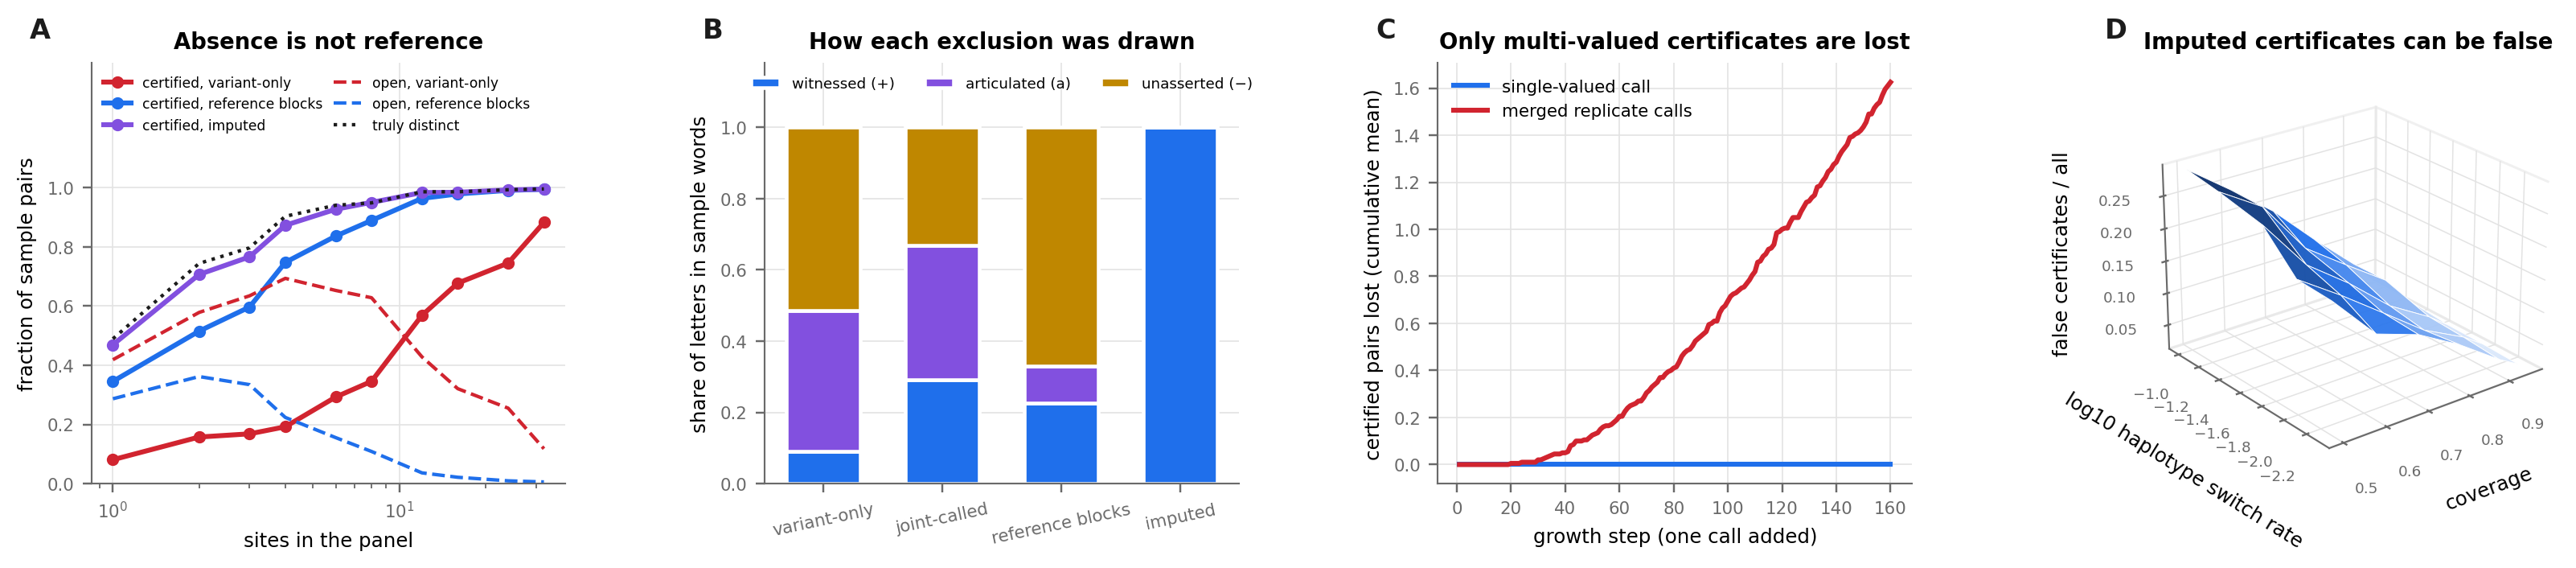
\includegraphics[width=\textwidth]{figures/panel_1_calls.png}
\caption{\textbf{Genotype calls as three-valued distinctions (E1).} A synthetic
cohort of $40$ samples with known genotypes (founder-mosaic haplotypes,
coverage $0.8$), emitted four ways (\Cref{def:emissions}).
(\textbf{A})~Fraction of sample pairs certified (solid) and open (dashed) against
the number of sites in the panel, eight replicates per point, with the fraction
truly distinct (dotted). Variant-only emission (red) certifies $19\%$ of pairs on
four sites, where reference blocks (blue) certify $75\%$ and $69\%$ remain open
under the former; the gap is \Cref{prop:vonly}. Imputation (purple) leaves no
pair open but certifies $87\%$ against $90\%$ truly distinct, and can certify
falsely.
(\textbf{B})~Letters of all sample words at $60$ sites
(\Cref{def:nest}). Under variant-only emission $51\%$ of exclusions are
unasserted ($\lm$); joint calling witnesses $29\%$; under imputation every
exclusion is witnessed ($\lp$), each witness for an imputed call being a
derivation.
(\textbf{C})~Certified pairs lost along $200$ random growth sequences of
$160$ steps: none for single-valued calls, $325$ for merged replicate calls,
as \Cref{thm:growth}(ii) requires.
(\textbf{D})~Rate of false certificates under imputation (certifying calls whose
true genotypes are equal) over coverage and haplotype switch rate: from
$0.21$--$0.29$ at coverage $0.5$ to $0.02$--$0.03$ at $0.95$. Under the three
truthful emissions the count is exactly $0$
(\Cref{prop:truthful}).}
\label{fig:p1}
\end{figure*}

\paragraph{Exhaustive checks.} Every assignment of $\{\cz,0/0,0/1,1/1\}$ to
three samples on one and two sites and to four samples on one and two sites was
enumerated: $69{,}952$ carvings and $407{,}232$ pairs. The status computed from
value sets and the status read off the distinctions agree on every pair
(\Cref{lem:status}); the three statuses partition the pairs ($247{,}752$
certified, $133{,}704$ open, $25{,}776$ indiscernible). Of $154{,}308$ chains in
the tolerance relation, $58{,}806$ fail transitivity, and $0$ of them do so
without an open link (\Cref{thm:trichotomy}).

\paragraph{The emission chain.} Over ten replicates of $40$ samples and $60$
sites, $0$ certified pairs were lost along $V\to J\to G\to I$
(\Cref{prop:chain}). Truthful emissions produced $0$ false certificates in every
replicate; imputation produced $17{,}070$ of $198{,}810$ certificates, and
$35.8\%$ of its certificates rest on at least one imputed value. Under
variant-only emission every absent non-reference call is undetermined ($1{,}604$
per replicate, $0$ witnessed reference); joint calling witnesses $48\%$ of them
and reference blocks $70\%$, the remainder being the uncovered positions
(\Cref{prop:vonly}). The sweep over panel size (\Cref{fig:p1}A) shows the same
on the pair level.

\paragraph{Non-locality.} Adding one call of another sample changed a sample's
word in $69$ of $600$ trials ($11.5\%$), although none of its own calls changed
(\Cref{prop:words}); its individuation changed in $1$.

% ---------------------------------------------------------------------
\subsection{E2: genericity and orbits}
\label{sec:e2}

\begin{figure*}[!t]
\centering
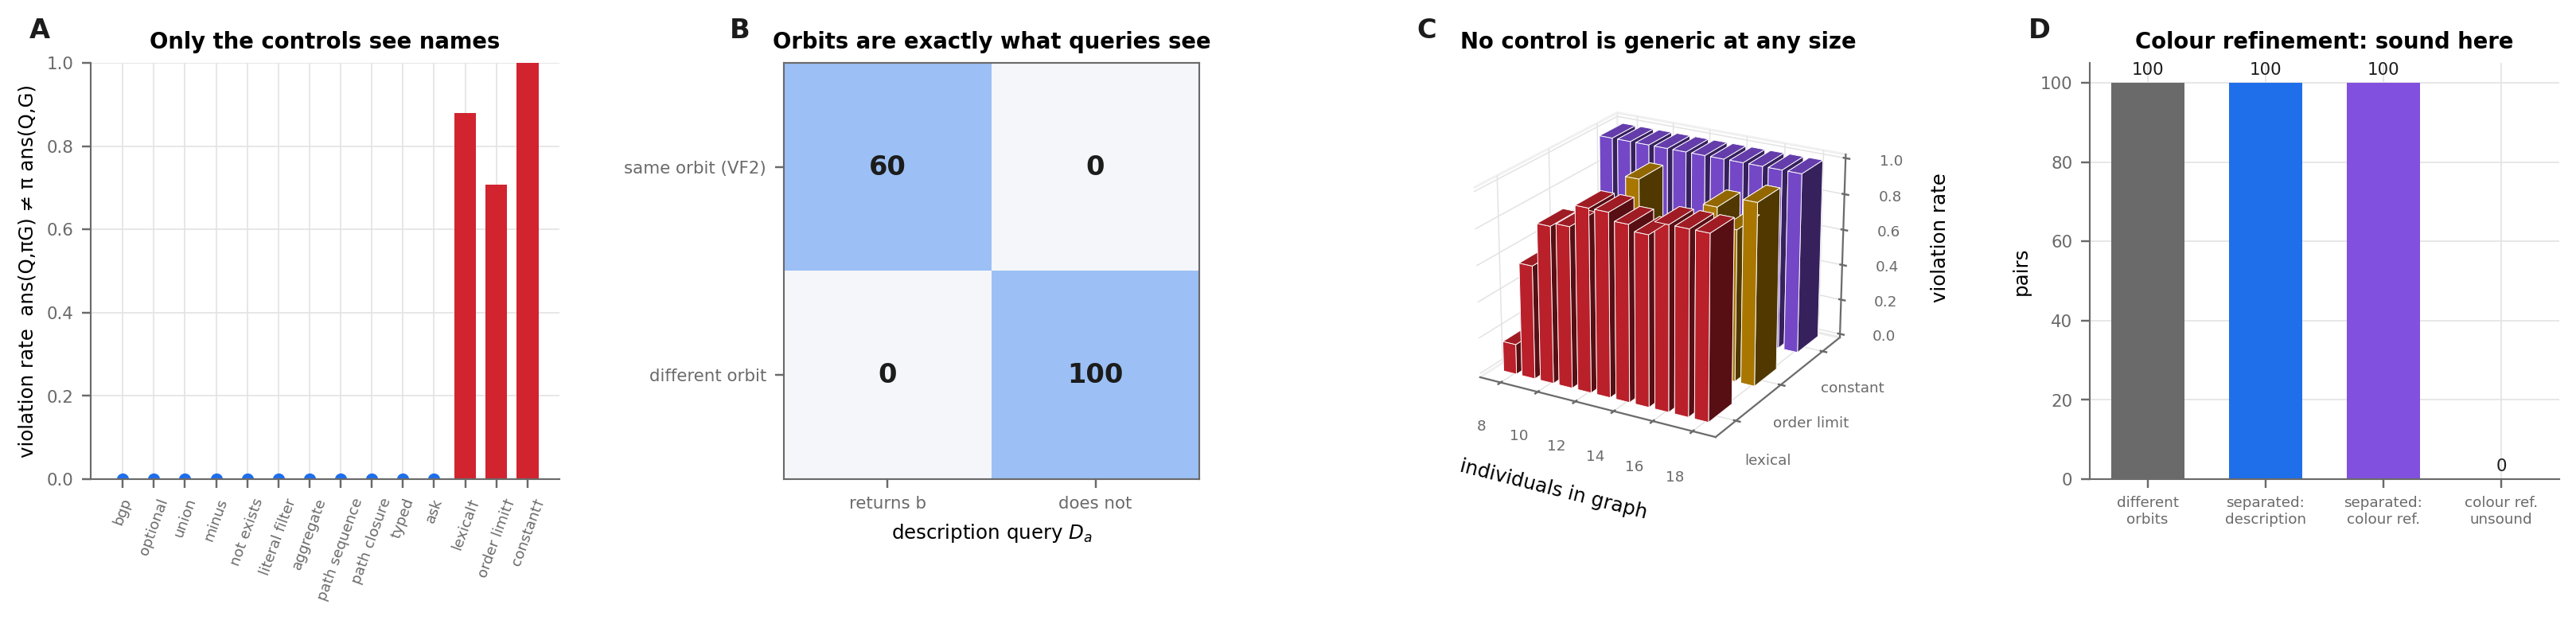
\includegraphics[width=\textwidth]{figures/panel_2_genericity.png}
\caption{\textbf{Identifier-blind queries over genomic provenance graphs (E2).}
Random graphs of samples, genotype calls, activities, inputs and agents ($8$--$18$
individuals).
(\textbf{A})~Violation rate of $\ans(Q,\pi G)=\pi\,\ans(Q,G)$ per query class,
$240$ tests each ($40$ graphs, six kind-preserving renamings). Eleven
identifier-blind classes show $0$ violations; the three controls ($\dagger$),
each lifting one exclusion of \Cref{def:frag}, violate genericity in $211$
(lexical comparison of identifiers), $170$ (ordering with truncation) and $240$
(a constant naming a call) of $240$ tests.
(\textbf{B})~Orbit characterisation on $160$ pairs from $40$ graphs with a planted
symmetry, half of them broken by one genotype literal: VF2 automorphism against
the description query $D_a$. The off-diagonal cells are $0$
(\Cref{thm:orbit}).
(\textbf{C})~Violation rate of the controls by graph size: none is generic at
any size.
(\textbf{D})~Of the $100$ pairs in different orbits, the description query and
colour refinement each separate $100$; colour refinement never separates a pair
within an orbit. Its completeness here is a property of the family, not of the
method \citep{cai1992}.}
\label{fig:p2}
\end{figure*}

Over $2{,}640$ tests in eleven classes---basic patterns, \texttt{OPTIONAL},
\texttt{UNION}, \texttt{MINUS}, \texttt{NOT EXISTS}, literal filters,
aggregation, sequence and closure paths, typed patterns and \texttt{ASK}---the
violation count is $0$ (\Cref{thm:generic}). The controls violate at $87.9\%$,
$70.8\%$ and $100\%$, so each exclusion is necessary. All $60$ pairs in one orbit
were returned by the description query and none of the $100$ pairs in different
orbits was. The description query is exponential in general (median $2.5$\,s,
maximum $234$\,s on these graphs); it characterises orbits and does not compute
them efficiently.

% ---------------------------------------------------------------------
\subsection{E3: receivers in published schemas}
\label{sec:e3}

\begin{figure*}[!t]
\centering
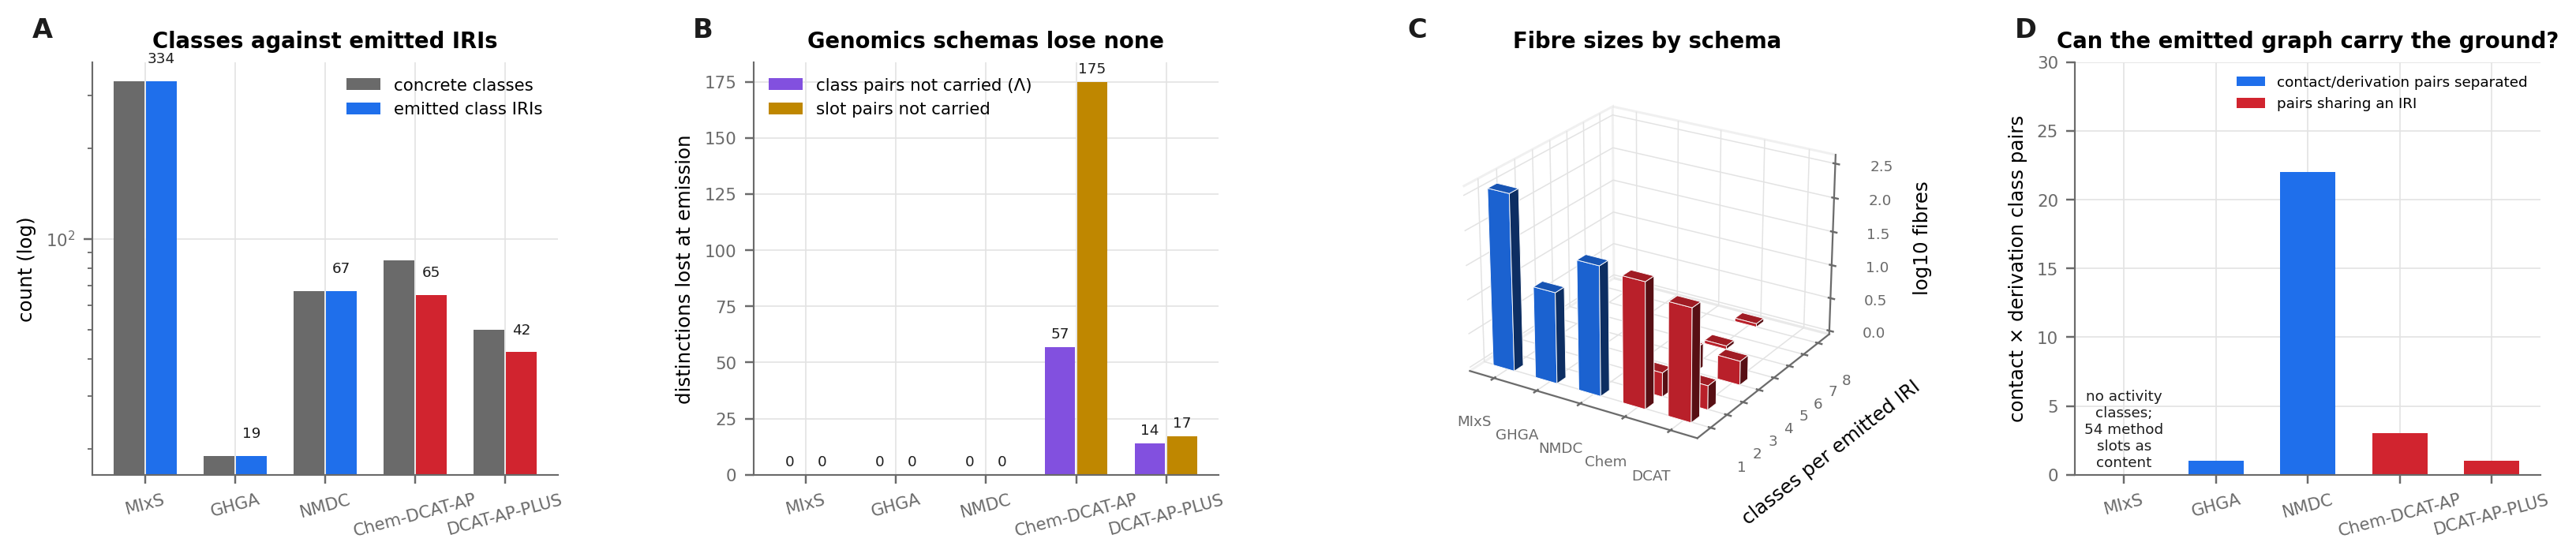
\includegraphics[width=\textwidth]{figures/panel_3_receivers.png}
\caption{\textbf{Receiver census of five LinkML schemas (E3).} Three genomics
schemas (blue) and two chemistry research-data profiles (red), read with their
imports closures at pinned commits.
(\textbf{A})~Concrete classes against emitted class IRIs (logarithmic). MIxS,
GHGA and NMDC emit $334$, $19$ and $67$ classes under as many IRIs;
Chem-DCAT-AP emits $85$ classes under $65$ IRIs and DCAT-AP-PLUS $50$ under
$42$.
(\textbf{B})~Class pairs whose distinction the type triple cannot carry
($\Lambda$, \Cref{prop:lambda}) and slot pairs sharing an emitted predicate:
$0$ and $0$ for every genomics schema; $57$ and $175$, and $14$ and $17$, for the
chemistry profiles.
(\textbf{C})~Distribution of fibre sizes (classes per emitted IRI) by schema.
Every genomics fibre is a singleton; the chemistry profiles have fibres of up
to eight classes, among them six activity classes emitted as
\texttt{prov:Activity}.
(\textbf{D})~Pairs of declared contact and derivation classes, and how many of
them share an IRI. GHGA (\texttt{Experiment} against \texttt{Analysis}) and NMDC
(two \texttt{DataGeneration} classes against eleven \texttt{WorkflowExecution}
classes) separate all of theirs; in the chemistry profiles every such pair
shares \texttt{prov:Activity}. MIxS declares no activity class at all and writes
method and software as values of $54$ content slots of the sample record.}
\label{fig:p3}
\end{figure*}

\Cref{tab:census} gives the census. The genomics schemas are injective
receivers at the level of class and predicate IRIs: no distinction a schema
draws by class is lost at emission ($\Lambda=0$). GHGA and NMDC are moreover
\emph{verdict-capable}: a processed file is linked to an \texttt{Analysis},
which is linked to the research data files it used, which are linked to an
\texttt{Experiment}, so the generation chain of a derived file reaches a
contact and its verdict is \vcom; NMDC's \texttt{WorkflowExecution} and
\texttt{DataGeneration} hierarchies play the same roles. MIxS is not
verdict-capable by construction: it describes samples, and writes the methods
that produced their data---\texttt{seq\_meth}, \texttt{assembly\_software},
\texttt{compl\_software} and $51$ further slots---as content of the sample. Ground
written as content is visible to content queries, but it is not a chain: it
cannot be followed to the record of another act, and two records whose method
slots differ are no longer twins at all. The chemistry profiles collapse every
activity class into \texttt{prov:Activity} (\Cref{thm:collapse}), so a
measured and a computed characterisation are written identically.

\begin{table}[t]
\centering\small
\caption{Receiver census. Concrete classes / emitted class IRIs, $\Lambda$, slots
/ emitted slot IRIs, slot pairs not carried, and whether declared contact and
derivation classes are separated.}
\label{tab:census}
\setlength{\tabcolsep}{3pt}
\resizebox{\columnwidth}{!}{\begin{tabular}{@{}lrrrrc@{}}
\toprule
Schema & classes & $\Lambda$ & slots & lost & capable\\
\midrule
MIxS & 334/334 & 0 & 1178/1178 & 0 & no class\\
GHGA & 19/19 & 0 & 108/108 & 0 & yes\\
NMDC & 67/67 & 0 & 875/875 & 0 & yes\\
Chem-DCAT-AP & 85/65 & 57 & 128/95 & 175 & no\\
DCAT-AP-PLUS & 50/42 & 14 & 99/87 & 17 & no\\
\bottomrule
\end{tabular}}
\end{table}

% ---------------------------------------------------------------------
\subsection{E4: verdicts on real annotation}
\label{sec:e4}

\begin{figure*}[!t]
\centering
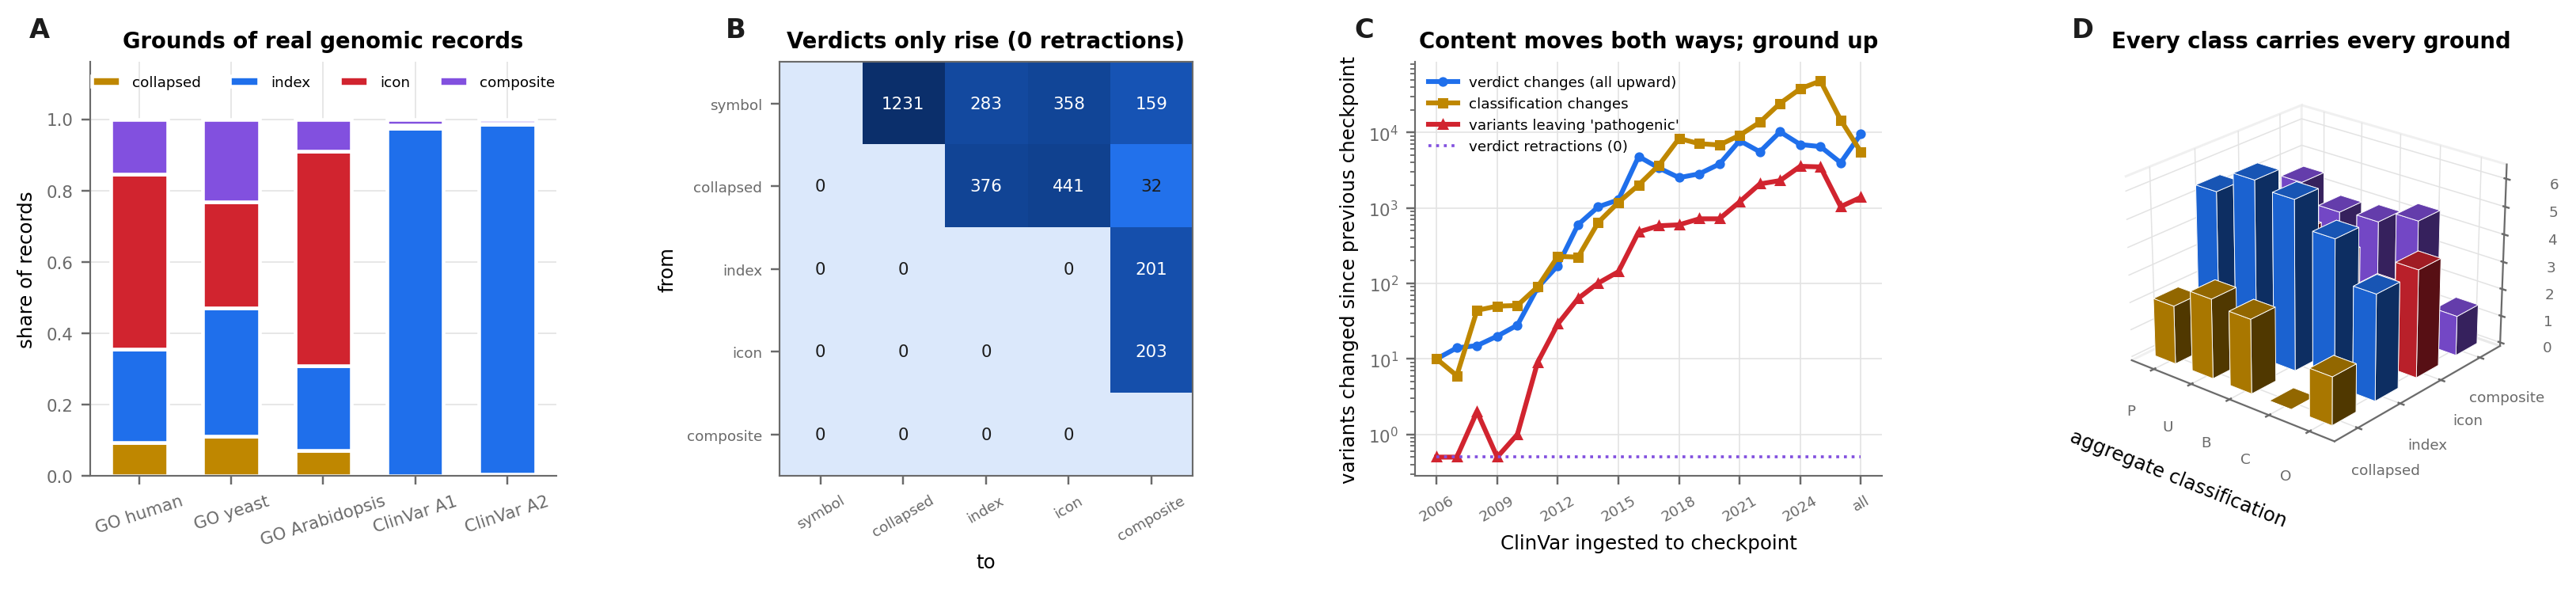
\includegraphics[width=\textwidth]{figures/panel_4_verdicts.png}
\caption{\textbf{Semiotic verdicts of real genomic records (E4).}
(\textbf{A})~Verdicts of gene--term memberships in three GO annotation sets and
of ClinVar variants under declarations A1 and A2 (\Cref{tab:declarations}).
Human memberships: $26\%$ \vind, $49\%$ \vico, $15\%$ \vcom, $9\%$ \vcol;
\emph{Arabidopsis}: $24\%$, $60\%$, $9\%$, $7\%$; yeast: $36\%$, $30\%$, $23\%$,
$11\%$. ClinVar variants are $97.4\%$ \vind{} under A1.
(\textbf{B})~Verdict transitions while $300$ synthetic provenance graphs with
generation chains grow triple by triple ($10{,}425$ additions, $3{,}284$
transitions): every transition goes up the order of \Cref{thm:monotone}, and
the count below the diagonal is $0$.
(\textbf{C})~ClinVar ingested in order of the date each submission was last
evaluated, at yearly checkpoints, logarithmic. Between consecutive checkpoints
$71{,}015$ variants changed verdict, all upward, while $183{,}585$ changed
aggregate classification and $18{,}493$ left the pathogenic class; verdict
retractions are $0$ throughout (plotted at $0.5$ on the logarithmic axis, as are
other zero counts).
(\textbf{D})~ClinVar variants by aggregate classification and verdict
(logarithmic): every classification occurs with every non-symbol verdict, the
real-data form of \Cref{prop:independent}.}
\label{fig:p4}
\end{figure*}

\paragraph{Census.} \Cref{tab:verdicts} gives the verdicts. The three GO
corpora differ sharply in ground: in \emph{Arabidopsis} $60\%$ of memberships
are supported only by derivation, against $30\%$ in yeast. Annotation lines
alone never have the verdict \vcom; memberships do, wherever experimental and
computational lines support the same gene and term
\citep{skunca2012}. In ClinVar the classifications differ in ground as well: of
$387{,}523$ variants whose submissions agree on \emph{pathogenic}, $85.8\%$ are
\vind, $5.8\%$ \vico{} and $8.4\%$ \vcom; of the $202{,}292$ with conflicting
classifications, $13.7\%$ are \vcom. Declaration A2 moves $23{,}994$ variants to
\vcol, $15{,}510$ of them pathogenic: the literature-only classifications
\citep{yang2017,harrison2017}.

\begin{table}[t]
\centering\small
\caption{Verdicts of real genomic records (counts).}
\label{tab:verdicts}
\setlength{\tabcolsep}{3pt}
\resizebox{\columnwidth}{!}{\begin{tabular}{@{}lrrrr@{}}
\toprule
 & \vcol & \vind & \vico & \vcom\\
\midrule
GO human & 31{,}224 & 88{,}174 & 165{,}338 & 52{,}105\\
GO yeast & 7{,}407 & 23{,}893 & 19{,}797 & 15{,}411\\
GO \emph{Arabidopsis} & 12{,}992 & 43{,}178 & 109{,}412 & 16{,}304\\
ClinVar A1 & 1{,}433 & 4{,}288{,}116 & 38{,}949 & 76{,}250\\
ClinVar A2 & 25{,}427 & 4{,}315{,}868 & 14{,}955 & 48{,}498\\
\bottomrule
\end{tabular}}
\end{table}

\paragraph{Definability.} The fixed-point ground and the ground read by the
three SPARQL queries of \Cref{lst:verdict} agree on $2{,}400/2{,}400$ synthetic
records with generation chains (all five verdicts present: $349$, $388$, $488$,
$648$, $527$), on $1{,}500/1{,}500$ human GO memberships and on
$1{,}500/1{,}500$ ClinVar variants emitted as RDF; both agree with the verdict
computed directly from the evidence codes and collection methods
(\Cref{thm:definable}).

\paragraph{Monotonicity.} No verdict fell in $10{,}425$ synthetic additions or in
any of $22$ ClinVar ingestion steps (\Cref{thm:monotone}). Content behaves
otherwise: $117{,}816$ variants moved from uncertain significance to
conflicting, $44{,}031$ from benign and $18{,}493$ from pathogenic. An answer to
``pathogenic variants in gene X'' can lose rows as submissions arrive; a stored
verdict is a valid lower bound forever. The ingestion order is a proxy for
history---each submission is represented by its current version---but the
theorem holds for every order.

\paragraph{Content independence.} Among $49{,}910$ groups of ClinVar variants
sharing a gene and an aggregate classification, every ordered pair of the four
non-symbol verdicts is realised in some group (\Cref{prop:independent}).

\paragraph{A VCF-style receiver.} Emitting only the aggregate classification and
the review status, as the INFO fields of a ClinVar VCF do, leaves $23$ emitted
classes, all but a negligible share of variants ($0.9999964$) in classes that
mix verdicts. The emitted fields retain $0.082$ of the $0.203$ bits of verdict
entropy per variant. The review status we emit is our aggregation (the
highest rank among a variant's submissions), not ClinVar's own field.

% ---------------------------------------------------------------------
\subsection{E5: twins}
\label{sec:e5}

\begin{figure*}[!t]
\centering
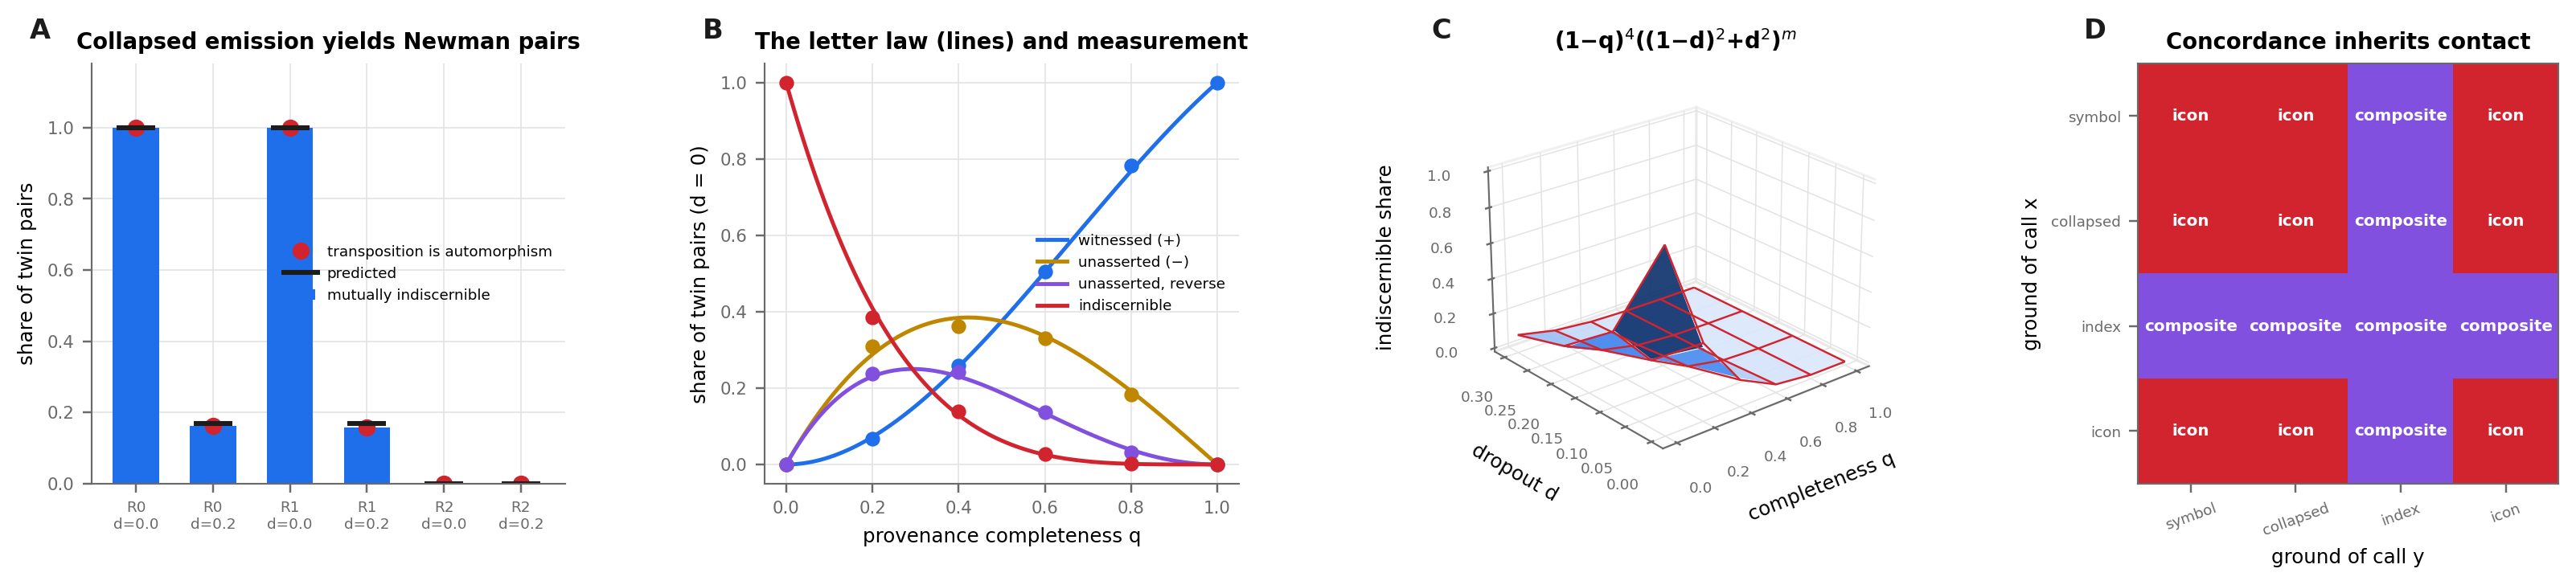
\includegraphics[width=\textwidth]{figures/panel_5_twins.png}
\caption{\textbf{A sequenced and an imputed genotype call with equal content
(E5).} $1{,}080$ twin pairs per setting.
(\textbf{A})~Share of pairs mutually indiscernible under the type projection
(bars), whose transposition is an automorphism of the emitted graph (red
markers), and predicted (black), under R0, R1, R2 (\Cref{def:regimes}) without
and with content dropout $d=0.2$. Collapsed emission (R0, R1) makes every
equal-content pair a Newman pair; typed activities (R2) separate all of them.
The two measures coincide in every pair of every setting.
(\textbf{B})~Under R3 with $d=0$: indiscernible pairs and the three kinds of
separation against provenance completeness $q$, measured (markers) and by the
law of \Cref{prop:twinprob} (lines). At $q=0.2$, $87\%$ of separations are
unasserted.
(\textbf{C})~Indiscernible share over $q$ and $d$, measured (surface) against
$(1-q)^4((1-d)^2+d^2)^m$ (wireframe).
(\textbf{D})~Verdict of a concordance record comparing two calls, by the
verdicts of the calls: it is \vcom{} exactly when one compared call has contact,
otherwise \vico{} (\Cref{prop:corrob}); $0$ violations in $2{,}000$ records.}
\label{fig:p5}
\end{figure*}

Under R0 and R1 with $d=0$ all $1{,}080$ pairs are orbit twins; under R2 none is,
and every separation carries the letter $\lp$ (\Cref{prop:r01,prop:r2}). With
$d=0.2$ the law predicts $181.7$ indiscernible pairs; R0 gives $176$ and R1
$169$. \Cref{tab:twinlaw} compares the law under R3 with the measurement. Mutual
indiscernibility and automorphism of the transposition disagreed in $0$ pairs
over all $30$ settings.

\begin{table}[t]
\centering\small
\caption{The twin law under R3, $d=0$, $1{,}080$ pairs: measured / predicted.}
\label{tab:twinlaw}
\setlength{\tabcolsep}{3pt}
\resizebox{\columnwidth}{!}{\begin{tabular}{@{}lrrrr@{}}
\toprule
$q$ & indiscernible & $\lp$ & $\lm$ & $\lm^{\mathrm{rev}}$\\
\midrule
0.2 & 417 / 442.4 & 73 / 77.8 & 334 / 311.0 & 256 / 248.8\\
0.4 & 149 / 140.0 & 279 / 276.5 & 391 / 414.7 & 261 / 248.8\\
0.6 & 29 / 27.6 & 546 / 544.3 & 357 / 362.9 & 148 / 145.2\\
0.8 & 2 / 1.7 & 846 / 829.4 & 197 / 207.4 & 35 / 41.5\\
1.0 & 0 / 0 & 1080 / 1080 & 0 / 0 & 0 / 0\\
\bottomrule
\end{tabular}}
\end{table}

% ---------------------------------------------------------------------
\subsection{E6: receivers of a sequence}
\label{sec:e6}

\begin{figure*}[!t]
\centering
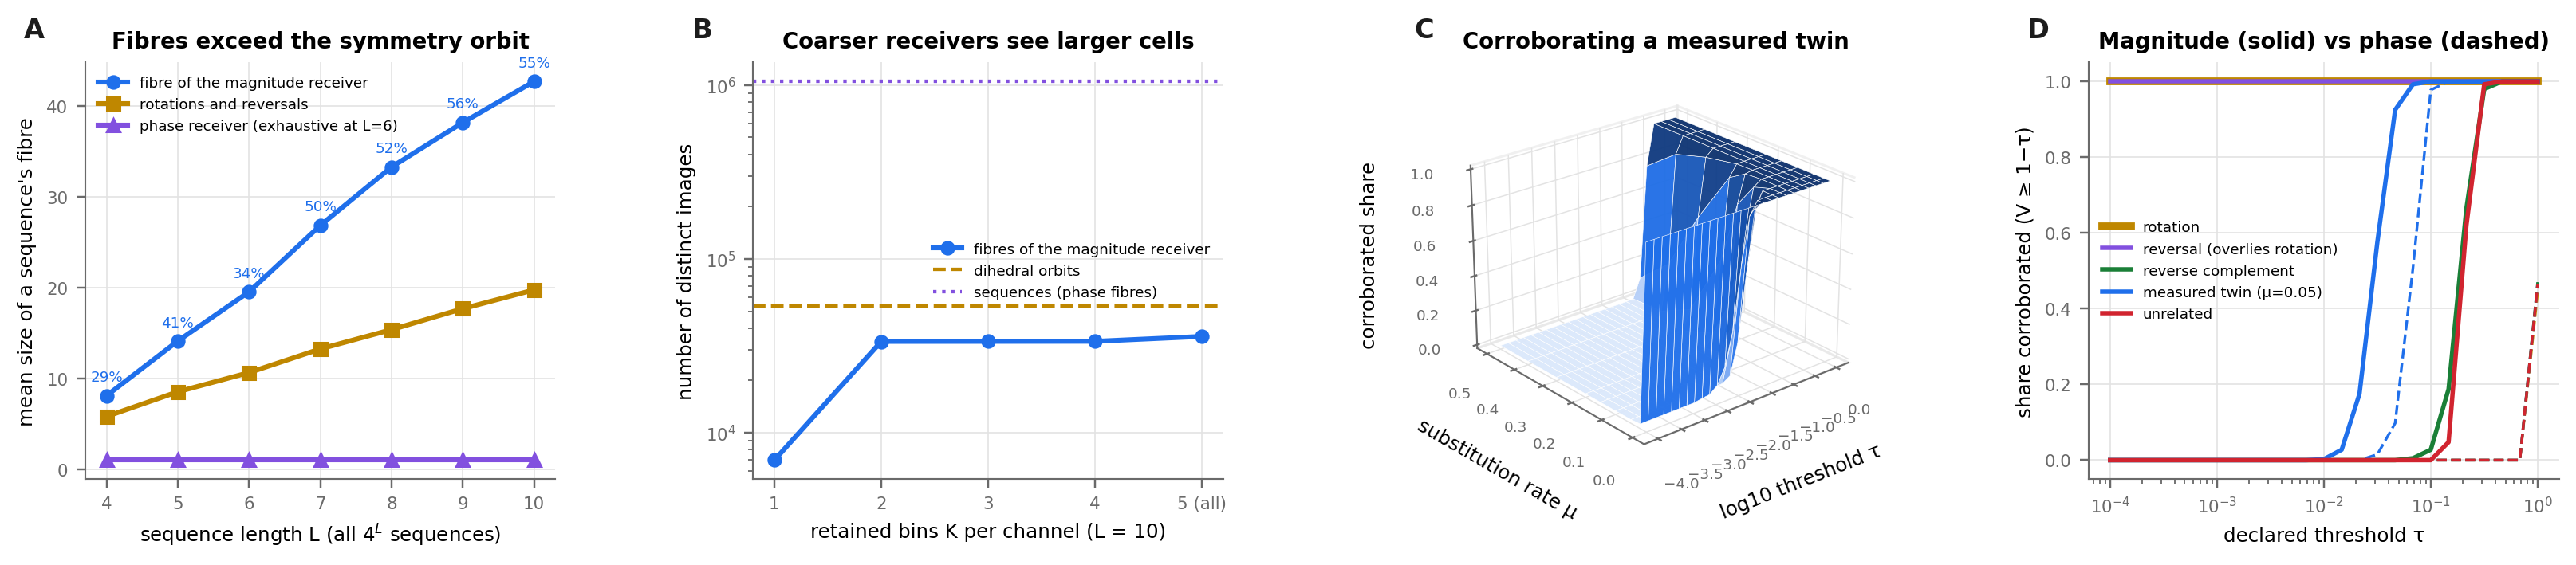
\includegraphics[width=\textwidth]{figures/panel_6_spectral.png}
\caption{\textbf{Identity at a declared floor (E6).}
(\textbf{A})~Exhaustively over all non-homopolymeric sequences of length
$L=4,\dots,10$ ($1{,}048{,}572$ at $L=10$): mean size of a sequence's fibre under
the full magnitude receiver, against the mean size of its dihedral orbit
(rotations and rotated reversals). Every orbit lies in one fibre ($0$
violations, \Cref{thm:dihedral}); labels give the share of sequences whose fibre
is strictly larger, $29\%$ at $L=4$ and $55\%$ at $L=10$. The phase receiver
has singleton fibres (\Cref{thm:phase}; exhaustive at $L=6$, $0$ of
$8{,}370{,}186$ pairs at visibility $1$).
(\textbf{B})~Number of distinct images at $L=10$ as the magnitude receiver keeps
$K=1,\dots,5$ bins per channel: $6{,}950$, $33{,}478$, $33{,}502$, $33{,}538$
and $35{,}790$, against $53{,}760$ dihedral orbits and $1{,}048{,}572$
sequences. Coarser receivers see larger cells (\Cref{prop:factor}).
(\textbf{C})~Share of measured twins (substitution rate $\mu$) of $400$ random
reference sequences of length $300$ corroborated by the magnitude receiver with
$K=12$, over the declared threshold $\tau$ and $\mu$.
(\textbf{D})~Corroboration rate against $\tau$ under the magnitude receiver
(solid) and the phase receiver (dashed). Rotations and reversals are
corroborated at every $\tau$ by magnitude and never by phase; reverse
complements and unrelated sequences become corroborated by magnitude only above
$\tau\approx0.1$, where all twins at $\mu=0.05$ already are.}
\label{fig:p6}
\end{figure*}

\Cref{tab:fibres} gives the exhaustive fibres. At every length the number of
magnitude fibres is smaller than the number of dihedral orbits---$35{,}790$
against $53{,}760$ at $L=10$---so the fibres merge orbits: more than half of
all sequences of length $8$--$10$ share their magnitude image with a sequence
that is neither a rotation nor a reversal of them. On sequences of length $300$
with $K=12$, measured twins at $\mu=0.05$ have median magnitude visibility
$0.971$ (minimum $0.912$) and unrelated sequences at most $0.896$; at
$\tau=0.1$ all twins and no unrelated sequence are corroborated, together with
every rotation and every reversal, and $2.8\%$ of reverse complements. The
strand receiver corroborates every reverse complement at every $\tau$
(\Cref{prop:strand}) and pays for it with a coarser view: unrelated sequences
reach $0.961$ and $27\%$ are corroborated at $\tau=0.1$. The phase receiver
places rotations, reversals and reverse complements near zero (at most
$0.156$).

\begin{table}[t]
\centering\small
\caption{Exhaustive fibres of the full magnitude receiver: sequences, fibres,
dihedral orbits, share of sequences in a fibre strictly larger than their orbit,
largest fibre. Invariance violations: $0$ at every length.}
\label{tab:fibres}
\setlength{\tabcolsep}{4pt}
\begin{tabular}{@{}rrrrrr@{}}
\toprule
$L$ & sequences & fibres & orbits & share & max\\
\midrule
4 & 252 & 43 & 51 & 0.286 & 24\\
5 & 1{,}020 & 98 & 132 & 0.412 & 30\\
6 & 4{,}092 & 332 & 426 & 0.343 & 72\\
7 & 16{,}380 & 898 & 1{,}296 & 0.497 & 84\\
8 & 65{,}532 & 3{,}020 & 4{,}431 & 0.523 & 160\\
9 & 262{,}140 & 10{,}004 & 15{,}080 & 0.556 & 108\\
10 & 1{,}048{,}572 & 35{,}790 & 53{,}760 & 0.554 & 240\\
\bottomrule
\end{tabular}
\end{table}

% ---------------------------------------------------------------------
\subsection{E7: answers and their grounding profiles}
\label{sec:e7}

\begin{figure*}[!t]
\centering
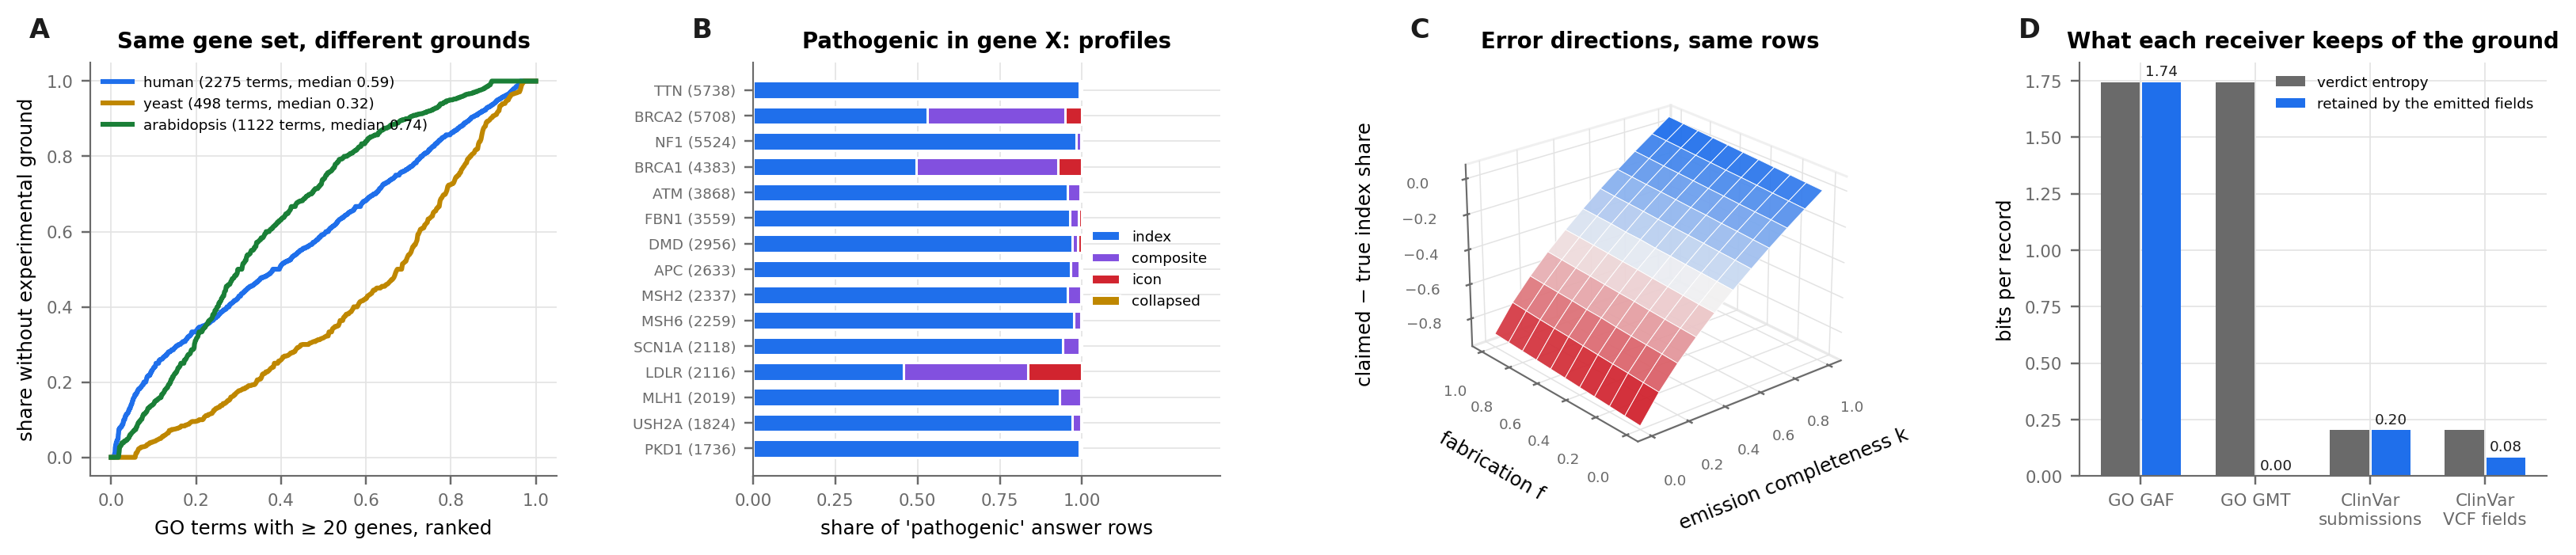
\includegraphics[width=\textwidth]{figures/panel_7_answering.png}
\caption{\textbf{Answers and grounding profiles on real annotation (E7).}
(\textbf{A})~For every GO term with at least $20$ member genes, the share of
members whose membership has no experimental ground (\vico{} or \vcol), terms
ranked. Medians: human $0.59$ ($2{,}275$ terms), yeast $0.32$ ($498$),
\emph{Arabidopsis} $0.74$ ($1{,}122$). A gene-set file returns the same members
for each term.
(\textbf{B})~Profiles of the answer ``variants classified pathogenic in gene X''
for the fifteen genes with most such variants. \emph{TTN} answers are $99\%$
\vind; \emph{BRCA2} $53\%$ \vind, $42\%$ \vcom, $5\%$ \vico; \emph{LDLR} $46\%$
\vind, $38\%$ \vcom, $16\%$ \vico.
(\textbf{C})~Claimed minus true index share (contact witness present) of the
$387{,}523$ pathogenic ClinVar variants, when each submission's collection method
is emitted with probability $k$ and a contact method is fabricated for variants
without one with probability $f$. Incomplete emission understates (to $-0.94$),
fabrication overstates (to $+0.06$, the whole remaining share), and the answer
rows are identical everywhere (\Cref{prop:directions}).
(\textbf{D})~Verdict information per record and the part each receiver keeps:
the GO annotation file keeps all $1.74$ bits of human memberships, a gene-set
file none; ClinVar submissions keep $0.20$ bits, VCF-style fields $0.08$.}
\label{fig:p7}
\end{figure*}

\paragraph{Gene sets.} In human, $60\%$ of GO terms with at least twenty genes
have a majority of members without experimental ground, and $3.6\%$ have none
with it; in \emph{Arabidopsis} $69\%$ and $10.4\%$; in yeast $32\%$ and $3.0\%$.
An enrichment analysis run on a gene-set file
\citep{subramanian2005,liberzon2011,khatri2012} receives the same members in
each case: the receiver is a function of the annotation file that forgets the
evidence (\Cref{prop:factor}), and the ground of every member becomes \vsym.
That enrichment results change with annotation releases is documented
\citep{tomczak2018}; the profile reported beside the answer says on what kind of
evidence each result rests.

\paragraph{Witnessed exclusions.} GO is almost entirely open-world in its
outside. Annotations qualified \texttt{NOT}, which witness that a gene does
\emph{not} have a function, number $1{,}383$ in human against $699{,}849{,}006$
absent gene--term memberships among the annotated genes and terms
($2.0\times10^{-6}$); $31$ in yeast and $1{,}087$ in \emph{Arabidopsis}. A
query for genes not annotated to a term returns, for all but a vanishing share,
genes about which nothing was asserted.

\paragraph{Profile freedom.} On $400$ real ClinVar variants emitted as content
graphs, $40$ random verdict assignments were realised by private provenance
gadgets. Four content queries---pathogenic variants, counts by gene, variants not
benign, conflicting or uncertain variants---returned identical bags in $40/40$
graphs, the verdicts read back by SPARQL matched the assignment in $40/40$, and
the profiles of the pathogenic answer differed by up to $0.44$ in total
variation (median $0.18$) (\Cref{thm:profilefree}).

% =====================================================================
\section{Discussion}
\label{sec:discussion}
% =====================================================================

\subsection{Four ways of being the same}

The question whether an imputed genotype ``is'' a called one, an electronic
annotation an experimental one, or a literature classification a clinical one
conflates four relations (\Cref{tab:same}). They are independent in the
directions that matter: content-same records can have any pair of grounds
(\Cref{prop:independent}, E4); orbit-same records are ground-same
(\Cref{thm:definable}) but not conversely; corroboration concerns sequences, not
graphs, and holds for records that differ in every other respect
(\Cref{cor:notidentity}). That a query returns two records alike is evidence of
content-sameness only, unless the query names provenance predicates.

\begin{table}[t]
\centering\small
\caption{Four sameness relations, what decides each, what can observe it.}
\label{tab:same}
\begin{tabular}{@{}L{0.22\columnwidth}L{0.33\columnwidth}L{0.35\columnwidth}@{}}
\toprule
Relation & Decided by & Observed by\\
\midrule
content-same & $\Desc_{\Pc}(r)=\Desc_{\Pc}(r')$ & content queries\\
orbit-same & an automorphism & all of $\Qfrag$; $D_r$\\
ground-same & $\gr(r)=\gr(r')$ & $Q_g,Q_c,Q_d$\\
corroborated & visibility $\ge1-\tau$ & a comparison record\\
\bottomrule
\end{tabular}
\end{table}

\subsection{The outside of a record}

The second half of the theory concerns what a record does not say. A cohort
emitted as variant-only files cannot witness a reference genotype
(\Cref{prop:vonly}); on a four-site panel it leaves $69\%$ of sample pairs open
that reference blocks certify. Imputation removes openness altogether, and in
doing so converts undetermined calls into derived ones: at coverage $0.5$ about
three quarters of its certificates rest on imputed values and a fifth to
three tenths of them are false. The pair status of the imputed cohort cannot
show this; the ground of its certifying calls can. GO shows the open world at
scale: two millionths of absent memberships are witnessed by \texttt{NOT}
annotations. In each case the information exists somewhere upstream---in the
alignments, in the panel, in the curators' judgements---and is lost or kept by
the receiver.

\subsection{Practices}

The theorems suggest six practices, none of which requires changing a query
language or an existing record.
\begin{enumerate}
\item \textbf{Emit reference blocks or joint calls, not variant-only files,} when
  absence must be read as reference (\Cref{prop:vonly}).
\item \textbf{Type imputed calls in the emitted graph.} A per-call imputation
  flag or a dosage field that survives merging is the second-typing remedy of
  R2; without it, imputed and called genotypes are Newman pairs
  (\Cref{prop:r01}).
\item \textbf{Carry evidence into gene sets.} A gene-set format that keeps the
  evidence code per member is a conservative extension of GMT, and lets the
  grounding profile of an enrichment be reported (\Cref{thm:profilefree}).
\item \textbf{Carry collection methods into variant files.} Classification and
  review status keep $40\%$ of the verdict information of ClinVar; the
  collection methods keep all of it (E4).
\item \textbf{Store verdicts as lower bounds; store cells, words and
  classifications with their stage.} Verdicts never fall
  (\Cref{thm:monotone}); classifications and words do (E4, E1).
\item \textbf{Declare the receiver of a sequence comparison.} A spectral
  sketch corroborates rotations, reversals and homometric sequences at every
  threshold; a strand receiver adds reverse complements; only the phase
  receiver identifies (\Cref{sec:floor}).
\end{enumerate}

\subsection{Relation to existing work}

The verdict calculus is a coarse, monotone, query-definable summary in the
programme of data provenance \citep{buneman2001,green2007,cheney2009}; finer
annotations (instrument, software version, reference panel) can be carried in
the same chains without changing any theorem. The three-valued calculus
continues the treatment of incomplete information in databases
\citep{codd1979,imielinski1984,libkin2016,reiter1978} and rough sets
\citep{pawlak1982,kryszkiewicz1998}. The evidence codes of GO and the Evidence
\& Conclusion Ontology \citep{giglio2019} are, in these terms, witness
declarations that the community already maintains; the quality of computational
annotation \citep{skunca2012,schnoes2009} and the discordance of clinical
classifications \citep{yang2017,harrison2017} are questions about content that
the ground makes reportable beside every answer. Genomic metadata standards
\citep{field2008,yilmaz2011,sansone2012,eloefadrosh2022} and data-sharing
frameworks \citep{rehm2021,wagner2021,wilkinson2016} fix what a graph can carry;
E3 measures it. The debate between simulation and experiment
\citep{morrison2009,parker2009,guala2002,morgan2005} is located: the equivalence
side is right about content (\Cref{cor:contentblind}), the materiality side is
right about ground (\Cref{thm:definable,prop:independent}), and neither states
that ground survives only where it is written.

% =====================================================================
\section{Limitations}
\label{sec:limits}
% =====================================================================

\begin{enumerate}[label=\textbf{L\arabic*.},leftmargin=2.2em]
\item \textbf{Declarations are inputs.} Which evidence codes and collection
  methods count as contact or derivation is declared, not derived; a second
  ClinVar declaration moves $23{,}994$ variants. The theorems hold for every
  declaration.
\item \textbf{Truthfulness is not checkable from the graph.} Soundness
  (\Cref{cor:sound}) assumes that the emission is contained in the true
  history; under fabrication verdicts are wrong in the direction that matters.
\item \textbf{The cohort is synthetic.} E1 and E5 need known genotypes and are
  run on a founder-mosaic simulation with a nearest-neighbour imputer; the
  closed forms are tested exactly, but the false-certificate rates of real
  imputation servers \citep{das2016,browning2016} are not estimated.
\item \textbf{ClinVar ingestion is a reconstruction.} Submissions are ordered by
  the date of last evaluation of their current versions, not by their history;
  the aggregate classification and the emitted review status are our rules, not
  ClinVar's. The monotonicity of verdicts holds for every order; the counts of
  reclassification are specific to this one.
\item \textbf{Memberships are direct.} GO memberships use direct annotations
  only, without propagation along the ontology, and NOT annotations are counted
  but not propagated.
\item \textbf{The fragment is not the language practitioners write.} Real
  queries name records, sort and truncate; the fragment isolates what a query
  can ask about structure.
\item \textbf{The description query is exponential} (up to $234$\,s on graphs
  of $18$ individuals). It characterises orbits; it is not an algorithm for them.
\item \textbf{Spectral models are idealised.} The receivers are the one-hot
  Fourier embeddings of alignment-free search; the exhaustive fibre counts stop
  at $L=10$.
\end{enumerate}

% =====================================================================
\section{Conclusion}
\label{sec:conclusion}
% =====================================================================

A sequenced genotype and an imputed one, an experimental annotation and an
electronic one, a clinical classification and a literature one: each pair is
the same in exactly one respect, its content, and every query in the vocabulary
of content answers it alike (\Cref{cor:contentblind}). Whether every structural
query answers it alike is decided by the emitted graph: the members are
inseparable exactly when they lie in one automorphism orbit (\Cref{thm:orbit}),
which happens whenever the receiver collapses their generating activities or
the emission omits what would tell them apart (\Cref{prop:r01,prop:twinprob}).

The other respect, their ground, is real. It is a structural property, defined
by three identifier-blind queries (\Cref{thm:definable}), monotone under the
growth of the graph (\Cref{thm:monotone}), sound under truthful emission
(\Cref{cor:sound}), and independent of content (\Cref{prop:independent}). On
real data it differs from term to term and from gene to gene, and the common
exchange formats keep little of it. The outside of a record is real too: a
variant-only file cannot say that a sample is reference, imputation fills the
silence with derivations, and an annotation database witnesses almost nothing
of what genes do not do. Between a read and a reference, identity is available
only through a receiver injective enough to give it, and a magnitude spectrum is
not. Each of these is a statement about what is written, and the practices of
\Cref{sec:discussion} are ways of writing it.

\paragraph{Data and code availability.} The validation suite is in
\texttt{validation/}: \texttt{fetch\_data.py} retrieves the public inputs and
records their digests, \texttt{e1\_calls.py}--\texttt{e7\_answering.py} write
\texttt{results/E*.json}, and \texttt{make\_panels.py} renders every figure from
those files alone; \texttt{run\_all.py} runs everything. The GO annotations are
those generated on 20--21 May 2026; the ClinVar submission summary was retrieved
on 3 October 2026; schema commits are listed in the bibliography.

\paragraph{Conflicts of interest.} None declared.

\bibliography{references}

\end{document}
